\documentclass[11pt,a4paper]{article}

% ===================== PACOTES =====================
\usepackage[utf8]{inputenc}
\usepackage[T1]{fontenc}
\usepackage[brazilian]{babel}
\usepackage[margin=2.1cm,top=2cm,bottom=2.2cm]{geometry}
\usepackage{graphicx}
\usepackage{booktabs}
\usepackage{float}
\usepackage{amssymb}
\usepackage{caption}
\usepackage{xcolor}
\usepackage{listings}
\usepackage{array}
\usepackage{multirow}
\usepackage{enumitem}
\usepackage{setspace}
\usepackage{amsmath}

\usepackage{siunitx}
\sisetup{
  locale = DE
}

% Por algum motivo esse precisa ficar por último
\usepackage[colorlinks=true,
            urlcolor=blue,
            linkcolor=blue,
            citecolor=black,
            backref=page]{hyperref}
            
% Changes URL links to a web-safe blue
\hypersetup{
    urlcolor=[HTML]{1155CC},
    linkcolor=blue,
    citecolor=black
}

% Texto do backref em português
\renewcommand{\backrefpagesname}{Citado na(s) p.}
\renewcommand{\backref}[1]{}
\renewcommand{\backrefalt}[4]{%
  {\footnotesize\sffamily
   [\ifcase #1 Não citado%
    \or Citado na p.~#2%
    \else Citado nas pp.~#2%
    \fi]}%
}

\captionsetup{font=small,labelfont=bf}

% ===================== CONFIGURAÇÃO DE CÓDIGO =====================
\definecolor{codebg}{rgb}{0.96,0.96,0.96}
\lstset{
    backgroundcolor=\color{codebg},
    basicstyle=\ttfamily\footnotesize,
    breaklines=true,
    frame=single,
    language=Python,
    showstringspaces=false,
    columns=fullflexible,
    keywordstyle=\color{blue},
    commentstyle=\color{gray}
}

\setlength{\parskip}{0.3em}
\setlength{\parindent}{0pt}
\setlength{\textfloatsep}{8pt plus 2pt minus 2pt}
\setlength{\floatsep}{6pt plus 2pt minus 2pt}
\setlength{\intextsep}{8pt plus 2pt minus 2pt}
\setlength{\abovecaptionskip}{4pt}
\setlength{\belowcaptionskip}{2pt}

\begin{document}
\sloppy

\begin{titlepage}
\centering

\vspace*{1.0cm}

{\LARGE\bfseries
Estimando a Conformidade de SLAs em um Serviço de\\[0.2cm]
Vídeo sob Demanda via Regressão e Classificação
\par}

\vspace{0.6cm}

{\large
PGC308A: Tópicos Especiais em Sistemas de Computação 2 - Internet do Futuro
\par}

\vspace{1.2cm}

{\large
Anna Letycia Fernandes Reis - 12612CCP008\\[0.2cm]
João Pedro Ramires Esteves - 12522CCP018
\par}

\vspace{0.9cm}

{\large
Universidade Federal de Uberlândia (UFU)\\[0.15cm]
Programa de Pós-Graduação em Ciência da Computação
\par}

\vspace{0.8cm}

{\large
29 de junho de 2026
\par}

\vspace{1.0cm}

\begin{minipage}{0.88\textwidth}
    \centering
    \textbf{\large Resumo}
    
    \vspace{0.35cm}
    
    \small
    Este relatório apresenta a análise experimental do problema de estimação de conformidade com Acordos de Nível de Serviço (SLAs) em um serviço de \textit{Video on Demand} (VoD). O objetivo é estimar a taxa de quadros observada no cliente a partir de estatísticas coletadas no servidor e, em seguida, classificar cada observação como conforme ou violadora do SLA definido (taxa mínima de 18 quadros - \textit{frames} - por segundo). Foram executadas três etapas: i) exploração dos dados; ii) regressão linear para estimação da métrica de serviço; e  iii) regressão logística para classificação de conformidade. Os resultados mostram que a regressão linear atingiu NMAE (\textit{Normalized Mean Absolute Error}) de 10,39\%, abaixo do limite de 15\% estabelecido no enunciado, enquanto o melhor classificador logístico obteve ERR (\textit{Classification Error}) de 11,11\%, também satisfazendo o critério de acurácia. A análise dos gráficos e das tabelas indica que os erros se concentram principalmente nas regiões de transição entre regimes de operação do servidor, especialmente nas proximidades do limiar de SLA.
\end{minipage}

\vfill

\end{titlepage}

\tableofcontents
\newpage


\section{Introdução}


Serviços de telecomunicações e de Internet dependem, cada vez mais, de infraestruturas de nuvem distribuída, computação de borda, CDNs e arquiteturas de rede programáveis. Nesse contexto, garantir a qualidade de serviço (QoS) percebida pelo cliente exige mecanismos de observabilidade capazes de relacionar métricas internas da infraestrutura a indicadores de experiência do usuário. Um \emph{Service Level Agreement} (SLA) formaliza esse compromisso, definindo um limiar mínimo de desempenho que o provedor deve sustentar.

Este trabalho investiga a conformidade de um serviço de vídeo sob demanda (VoD) a um SLA definido em termos da taxa de quadros (\emph{frame rate}) observada no terminal do cliente. A abordagem proposta é orientada a dados: a partir de estatísticas do sistema operacional coletadas no servidor (CPU, memória, processos, rede etc.), constrói-se um modelo de aprendizado de máquina $M: X \rightarrow \hat{Y}$ capaz de estimar a métrica de serviço $Y$ sem a necessidade de instrumentar o lado do cliente. O problema é tratado tanto como regressão (estimação do valor contínuo da taxa de quadros) quanto como classificação binária (conformidade ou violação ao SLA), utilizando, respectivamente, regressão linear e regressão logística como modelos-base interpretáveis.

O restante do relatório está organizado da seguinte forma: a Seção~\ref{sec:dataset} descreve o conjunto de dados utilizado; a Seção~\ref{sec:taskI} apresenta a exploração estatística dos dados (Task~I); a Seção~\ref{sec:taskII} discute a estimação da taxa de quadros via regressão linear (Task~II); a Seção~\ref{sec:taskIII} apresenta o classificador de conformidade ao SLA via regressão logística (Task~III); e a Seção~\ref{sec:conclusao} sintetiza as conclusões do trabalho.


\section{Descrição do Conjunto de Dados}
\label{sec:dataset}


O conjunto de dados contém 3600 observações coletadas em intervalos de um segundo ao longo de uma hora de operação de um servidor de VoD. Cada observação relaciona nove estatísticas de dispositivo do servidor (variáveis explicativas $X$) à taxa de quadros exibida no cliente naquele instante (variável resposta $Y$). Por clareza de notação, as features originais foram renomeadas conforme a Tabela~\ref{tab:features}.

\begin{table}[H]
\centering
\caption{Dicionário de variáveis do conjunto de dados.}
\label{tab:features}
\begin{tabular}{llll}
\toprule
Variável original & Nome utilizado & Descrição & Unidade \\
\midrule
\texttt{all\_..idle} & \texttt{cpu.idle} & Percentual de tempo ocioso da CPU & \% \\
\texttt{X..memused} & \texttt{mem.used} & Percentual de memória utilizada & \% \\
\texttt{proc.s} & \texttt{proc.creation.rate} & Taxa de criação de processos & processos/s \\
\texttt{cswch.s} & \texttt{ctx.switch.rate} & Taxa de troca de contexto & trocas/s \\
\texttt{file.nr} & \texttt{file.handles} & Número de \textit{file handles} em uso & contagem \\
\texttt{sum\_intr.s} & \texttt{interrupt.rate} & Taxa de interrupções & interrupções/s \\
\texttt{ldavg.1} & \texttt{load.avg.1min} & \textit{Load average} no último minuto & adimensional \\
\texttt{tcpsck} & \texttt{tcp.sockets} & Número de sockets TCP em uso & contagem \\
\texttt{pgfree.s} & \texttt{pg.free.rate} & Taxa de liberação de páginas de memória & páginas/s \\
\texttt{DispFrames} & \texttt{frame.rate} & Taxa de quadros exibidos & frames/s \\
\bottomrule
\end{tabular}
\end{table}

O SLA do serviço é definido em termos do \emph{frame rate}: diz-se que o serviço \textbf{conforma} ao SLA em um instante se $Y \geq 18$ fps, e que \textbf{viola} o SLA caso contrário. Esse limiar é utilizado tanto na Task~II, como referência visual de qualidade, quanto na Task~III, como definição do rótulo binário a ser classificado.


\section{Task I - Exploração dos Dados}
\label{sec:taskI}


\subsection{Estatísticas Descritivas}

A primeira etapa consistiu em calcular, para cada variável de \(X\) e para a variável \(Y\), média, desvio padrão amostral, mínimo, percentil 25, percentil 90 e máximo. Os cálculos foram realizados de duas formas, uma com NumPy e outra com Pandas, e os resultados foram comparados por meio de verificação cruzada, confirmando que ambos os métodos produziram resultados idênticos. A Tabela~\ref{tab:stats} resume os valores obtidos.

\begin{table}[H]
\centering
\caption{Estatísticas descritivas das variáveis do conjunto de dados.}
\label{tab:stats}
\small
\begin{tabular}{lrrrrrr}
\toprule
\textbf{Variável} & \textbf{Média} & \textbf{Desvio} & \textbf{Mín.} & \textbf{P25} & \textbf{P90} & \textbf{Máx.} \\
\midrule
cpu.idle (\%)              & 9.06     & 16.122   & 0.00    & 0.00     & 38.62    & 69.54 \\
mem.used (\%)              & 89.13    & 8.18     & 73.03   & 82.96   & 96.77    & 97.84 \\
proc.creation.rate         & 7.68     & 8.53     & 0.00     & 0.00     & 20.00    & 48.00 \\
ctx.switch.rate            & 54,045.87 & 19,497.81 & 11,398.00 & 31,302.00 & 72,135.10 & 83,880.00 \\
file.handles               & 2,656.33  & 196.11   & 2,304.00  & 2,496.00  & 2,880.00  & 2,976.00 \\
interrupt.rate             & 19,978.04 & 4,797.27  & 10,393.00 & 16,678.00 & 28,228.40 & 35,536.00 \\
load.avg.1min              & 75.87    & 43.86    & 11.13    & 28.20    & 127.99   & 147.47 \\
tcp.sockets                & 48.99    & 15.87    & 21.00    & 34.00    & 71.00    & 87.00 \\
pg.free.rate                & 72,872.15 & 19,504.32 & 15,928.00 & 61,601.75 & 97,532.50 & 145,874.00 \\
\textbf{frame.rate (Y)}    & \textbf{18.81} & \textbf{5.21} & \textbf{0.00} & \textbf{13.39} & \textbf{24.61} & \textbf{30.39} \\
\bottomrule
\end{tabular}
\end{table}





A Tabela~\ref{tab:stats} mostra que o servidor opera, na maior parte do tempo, com alta utilização de recursos. O uso médio de memória é de 89{,}14\%, com o primeiro quartil em 82{,}97\% e o percentil 90 alcançando 96{,}77\%. Já a ociosidade média da CPU é de apenas 9{,}07\%, sendo que pelo menos 25\% das observações registram 0\% de CPU livre. Esse comportamento indica um ambiente frequentemente próximo da saturação. Além disso, a taxa média de quadros é de 18{,}82 fps, valor muito próximo ao limite de SLA de 18 fps, sugerindo que pequenas oscilações na carga podem ser suficientes para levar o sistema a situações de conformidade ou violação. Os desvios padrão elevados de \texttt{load.avg.1min} e \texttt{ctx.switch.rate} também indicam uma variação significativa na carga ao longo do tempo, aspecto que será explorado nas próximas análises.


\subsection{Consultas sobre o Conjunto de Dados}

Três consultas específicas foram realizadas sobre os dados, com o objetivo de quantificar condições de operação sob alta carga. Os resultados, calculados de forma equivalente via filtragem booleana em \texttt{NumPy} e em \texttt{pandas}, são apresentados na Tabela~\ref{tab:queries}.

\begin{table}[H]
\centering
\caption{Resultados das consultas sobre o conjunto de dados (3,600 observações).}
\label{tab:queries}
\begin{tabular}{lr}
\toprule
\textbf{Consulta} & \textbf{Resultado} \\
\midrule
(a) Observações com \texttt{mem.used} $>$ 80\% & 2,875 (79{,}86\%) \\
(b) Média de \texttt{tcp.sockets} quando \texttt{interrupt.rate} $>$ 18,000/s & 46{,}35 sockets \\
(c) Mínimo de \texttt{mem.used} quando \texttt{cpu.idle} $<$ 20\% & 73{,}03\% \\
\bottomrule
\end{tabular}
\end{table}

O item (a) confirma que a alta ocupação de memória é uma condição frequente do servidor: 2875 das 3600 observações, superando os 80\% em quase 80\% do tempo monitorado. Já o item (b) mostra que, mesmo sob tráfego intenso com mais de 18.000 interrupções por segundo, o número médio de \emph{sockets} TCP ativos (46{,}35) permanece muito próximo da média global (48{,}99), indicando que a quantidade de conexões TCP não varia diretamente com a taxa de interrupções. Por fim, o item (c) reforça esse cenário de sobrecarga ao evidenciar que, mesmo nos momentos de menor ociosidade da CPU (abaixo de 20\%), o uso de memória nunca fica abaixo de 73{,}03\%, que corresponde ao menor valor observado para essa métrica em todo o conjunto de dados. Em conjunto, os resultados confirmam a caracterização de um ambiente que opera sob carga elevada durante a maior parte do tempo.

\subsection{Análise Gráfica}

\subsubsection{Série Temporal de CPU Idle e Memória Utilizada}

A Figura~\ref{fig:series} apresenta as séries temporais de \texttt{cpu.idle} e \texttt{mem.used} ao longo dos 3600 segundos de monitoramento, plotadas no mesmo eixo (ambas em \%).

\begin{figure}[H]
\centering
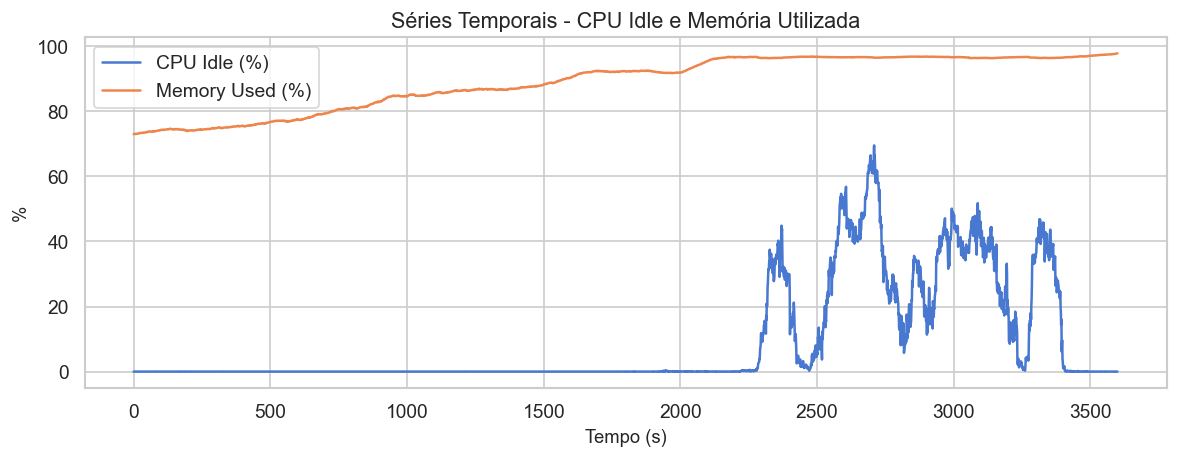
\includegraphics[width=0.85\textwidth]{figuras/fig_series_cpu_mem.png}
\caption{Séries temporais de CPU ociosa e memória utilizada.}
\label{fig:series}
\end{figure}


A série temporal mostra que CPU e memória apresentam comportamentos distintos ao longo do período analisado. Na primeira parte da coleta (aproximadamente do segundo 0 ao 2200), a CPU permanece praticamente saturada (\texttt{cpu.idle} $\approx 0\%$) enquanto a memória cresce de forma contínua de 73\% para perto de 97\%. A partir do segundo 2200, a CPU passa a apresentar picos intermitentes de ociosidade de até 70\%, enquanto a memória permanece estável em um patamar elevado, entre 96\% e 98\%. Esses resultados sugerem que o sistema opera sob carga elevada durante grande parte do tempo, com a memória mantendo níveis altos de utilização mesmo nos momentos em que a CPU apresenta algum alívio. Esse comportamento indica mudanças no regime de operação ao longo da coleta e ajuda a explicar parte da variabilidade observada nas demais métricas.

\subsubsection{Estimativas de Densidade (KDE)}

A Figura~\ref{fig:kde_cpu_mem} apresenta as estimativas de densidade de \emph{kernel} (KDE) para \texttt{cpu.idle} e \texttt{mem.used}, calculadas com \emph{kernel} Gaussiano e largura de banda definida pela regra de Silverman ($h^* = 1{,}06\, \hat{\sigma}\, n^{-1/5}$). As curvas obtidas pela implementação manual e pela função \texttt{KernelDensity} do \texttt{scikit-learn} coincidem exatamente, validando a implementação.

\begin{figure}[H]
\centering
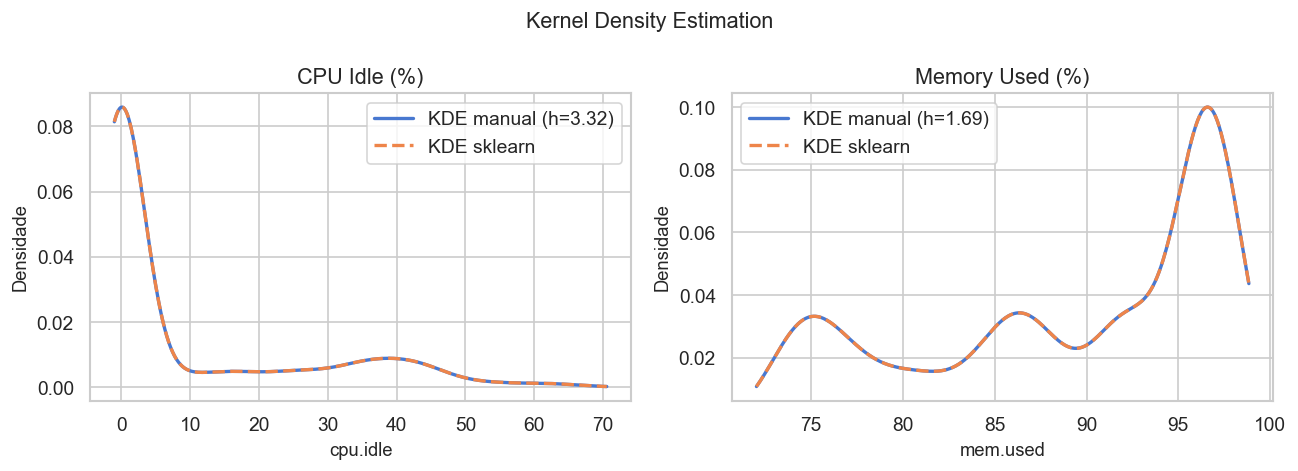
\includegraphics[width=\textwidth]{figuras/fig_kde_cpu_mem.png}
\caption{KDE de CPU ociosa (esquerda) e memória utilizada (direita).}
\label{fig:kde_cpu_mem}
\end{figure}

A análise do gráfico de densidade revela que a KDE de \texttt{cpu.idle} concentra massa próxima de zero, indicando que a CPU permaneceu com baixa ociosidade durante grande parte do período analisado. Embora existam observações com níveis mais elevados de ociosidade, elas ocorrem com menor frequência. Já a distribuição de \texttt{mem.used} concentra-se em valores altos e apresenta mais de uma região de maior densidade, com destaque para a faixa entre 96\% e 97\%. As duas curvas mostram que a memória permanece constantemente demandada, enquanto a CPU responde de forma mais dinâmica às variações da carga de trabalho.


\section{Task II - Estimação da Métrica de Serviço a partir das Estatísticas de Dispositivo}
\label{sec:taskII}


\subsection{Formulação e Divisão Treino/Teste}

Na Task II, o objetivo foi treinar um modelo de regressão linear múltipla \(M:X\rightarrow \hat{Y}\), em que \(X\) contém as nove estatísticas do dispositivo e \(Y\) corresponde ao \texttt{frame.rate}. O modelo ajustado tem a forma:
\begin{equation}
    \hat{y} = \theta_0 + \theta_1x_1 + \theta_2x_2 + \cdots + \theta_9x_9.
\end{equation}

Seguindo a técnica de \emph{validation-set}, o conjunto de 3600 observações foi particionado aleatoriamente em 70\% para treino (2520 observações) e 30\% para teste (1080 observações), utilizando \texttt{train\_test\_split} do \texttt{scikit-learn} com semente fixa (\texttt{random\_state=42}) para garantir reprodutibilidade:

\begin{lstlisting}
X_train, X_test, y_train, y_test = train_test_split(
    X, y, test_size=0.30, random_state=SEED
)
\end{lstlisting}

O modelo foi ajustado por Mínimos Quadrados Ordinários (OLS), utilizando essas nove estatísticas como variáveis explicativas.

\subsection{Avaliação da Acurácia de Estimação}

\subsubsection{Coeficientes do Modelo}

Inicialmente, foi treinado um modelo de regressão linear com o conjunto de treino completo (2520 observações). O intercepto obtido foi \(\theta_0=49,69\). A Tabela~\ref{tab:coef-linear-principal} apresenta os coeficientes ordenados por magnitude absoluta.

\begin{table}[H]
\centering
\caption{Coeficientes do modelo linear treinado com 2520 observações.}
\label{tab:coef-linear-principal}
\begin{tabular}{lrp{8cm}}
\toprule
Variável & Coeficiente & Interpretação \\
\midrule
\texttt{cpu.idle} & -0,0921 & Coeficiente de maior magnitude; o sinal negativo é contraintuitivo e sugere colinearidade com outras variáveis de carga. \\
\texttt{mem.used} & -0,0868 & Maior uso de memória está associado à redução do \textit{frame rate}. \\
\texttt{tcp.sockets} & -0,0653 & Mais conexões simultâneas estão associadas a maior sobrecarga. \\
\texttt{load.avg.1min} & -0,0606 & Maior carga média reduz a capacidade do servidor de manter a taxa de quadros. \\
\texttt{proc.creation.rate} & -0,0120 & Impacto menor, porém ainda negativo. \\
\texttt{file.handles} & -0,0031 & Impacto marginal. \\
\texttt{ctx.switch.rate} & -0,0001 & Efeito praticamente nulo na escala observada. \\
\texttt{interrupt.rate} & 0,0000 & Efeito negligenciável. \\
\texttt{pg.free.rate} & -0,0000 & Efeito negligenciável. \\
\bottomrule
\end{tabular}
\end{table}

A interpretação dos coeficientes indica que variáveis relacionadas à carga do sistema estão, em geral, associadas à redução da taxa de \emph{frame rate} estimada. O intercepto ($\theta_0 = 49{,}69$) representa o valor teórico do \emph{frame rate} na ausência de carga, servindo como um limite superior do modelo dentro da formulação linear. De forma consistente com a Tabela~\ref{tab:coef-linear-principal}, todos os coeficientes são negativos ou próximos de zero, sugerindo que o aumento no uso de recursos tende a degradar o desempenho. As variáveis \texttt{cpu.idle}, \texttt{mem.used}, \texttt{tcp.sockets} e \texttt{load.avg.1min} concentram os efeitos de maior magnitude, enquanto métricas como \texttt{ctx.switch.rate}, \texttt{interrupt.rate} e \texttt{pg.free.rate} apresentam impacto praticamente nulo na predição.

O coeficiente negativo de \texttt{cpu.idle} chama atenção, pois isoladamente seria esperado que mais CPU ociosa resultasse em uma taxa de \emph{frame rate} maior. Essa inversão é um forte indício de colinearidade entre as \emph{features}. Como as variáveis de memória, carga média e \emph{sockets} TCP já absorvem a maior parte da informação sobre a carga do servidor, o coeficiente de \texttt{cpu.idle} passa a refletir apenas um efeito residual condicional, e não o seu impacto isolado. Isso indica que os coeficientes devem ser interpretados em conjunto dentro do modelo, e não como efeitos causais independentes.


\subsubsection{Acurácia do Modelo (NMAE)}

O erro do modelo no conjunto de teste foi avaliado pelo Erro Absoluto Médio Normalizado (NMAE):

\begin{equation}
    \text{NMAE} = \frac{1}{\bar{y}} \left( \frac{1}{m} \sum_{i=1}^{m} \left| y_i - \hat{y}_i \right| \right)
\end{equation}

Os resultados obtidos foram: $\text{MAE} = 1{,}9371$ fps, $\bar{y} = 18{,}65$ fps (média da variável resposta no conjunto de teste) e, portanto, $\text{NMAE} = 0{,}1039$ ($10{,}39\%$). Como $10{,}39\% < 15\%$, o critério de acurácia estabelecido pelo enunciado é satisfeito, classificando o modelo como \textbf{acurado}.

\subsubsection{Série Temporal: Estimativas \emph{vs.} Medições}

A Figura~\ref{fig:series_pred} compara, no conjunto de teste, o \emph{frame rate} medido e a estimativa do modelo, apresentando as médias móveis de 30 segundos no painel superior para suavizar o ruído ponto-a-ponto e os resíduos individuais no painel inferior.

\begin{figure}[H]
\centering
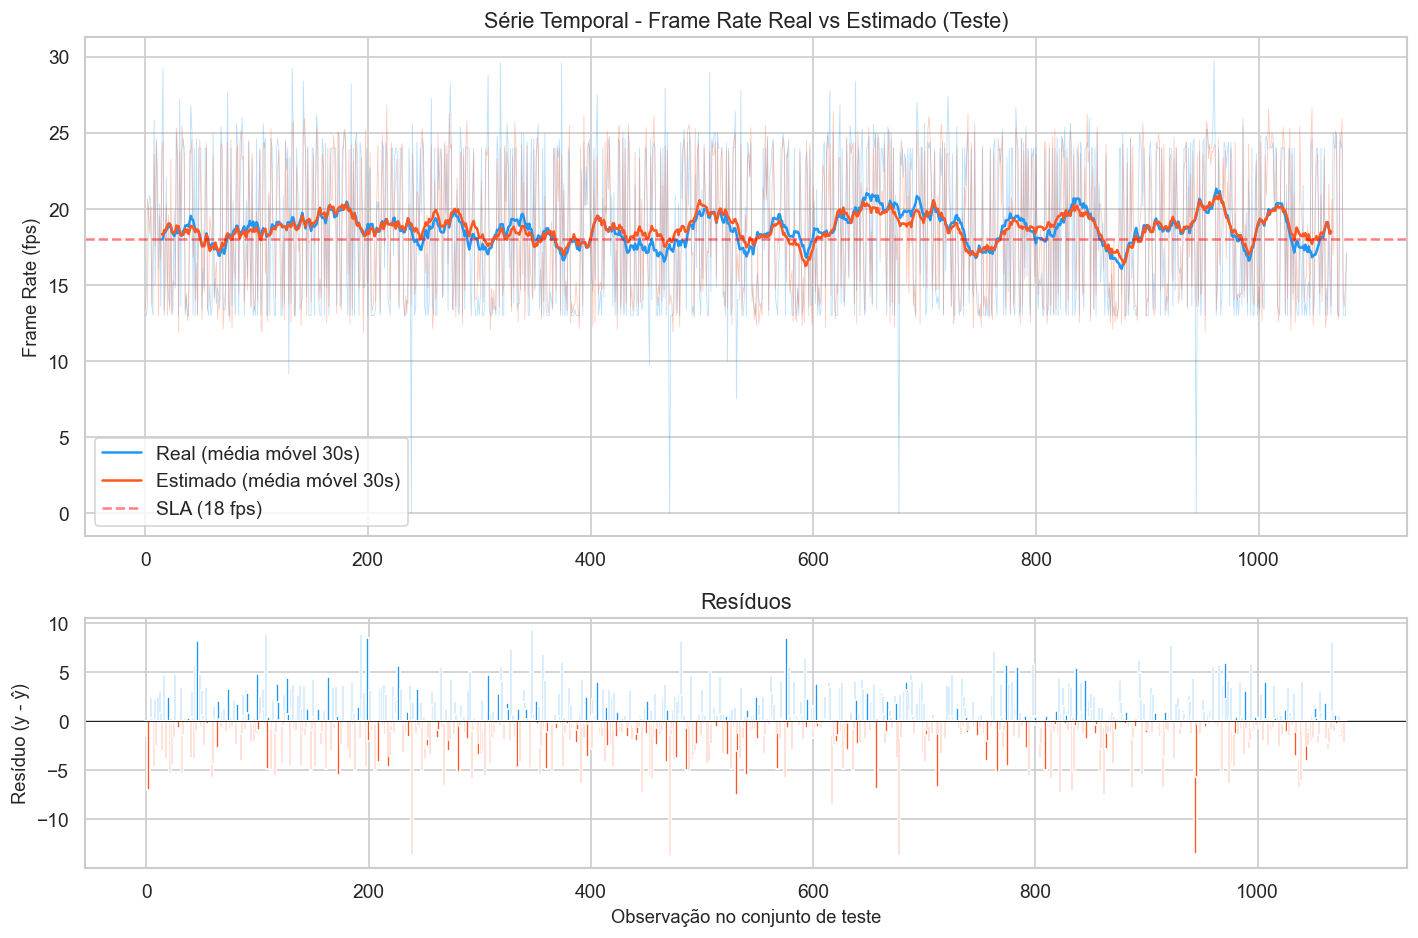
\includegraphics[width=0.95\textwidth]{figuras/fig_series_pred_real.png}
\caption{Série temporal do \emph{frame rate} real e estimado no teste, com resíduos.}
\label{fig:series_pred}
\end{figure}

A curva estimada acompanha bem o comportamento real ao longo de todo o conjunto de teste, capturando com precisão as oscilações de médio prazo em torno do limiar de SLA, representado pela linha pontilhada em 18 fps. As diferenças entre os valores reais e estimados permanecem pequenas na maior parte do tempo, embora ocorram picos isolados de erro de aproximadamente  $\pm 10$ fps em alguns pontos específicos. Esses casos coincidem com mudanças rápidas no comportamento do sistema, nas quais a regressão linear tende a suavizar as predições e não consegue acompanhar a velocidade da mudança do valor real.

\subsubsection{KDE do \emph{Frame Rate} no Conjunto de Teste}

A Figura~\ref{fig:kde_framerate} apresenta a KDE do \emph{frame rate} real no conjunto de teste, com indicação do limiar
de SLA de 18 fps.

\begin{figure}[H]
\centering
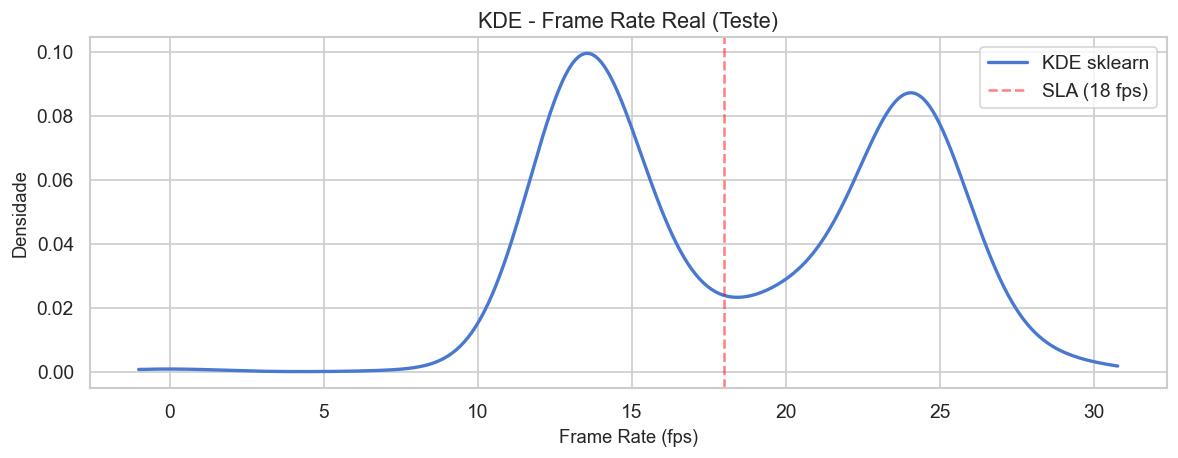
\includegraphics[width=0.8\textwidth]{figuras/fig_kde_framerate_test.png}
\caption{KDE do \emph{frame rate} real no conjunto de teste.}
\label{fig:kde_framerate}
\end{figure}

A distribuição do \emph{frame rate} no conjunto de teste é claramente \textbf{bimodal}, com dois picos bem definidos próximos de 13 fps e de 24 fps, e um vale exatamente sobre o limiar de SLA (18 fps). Isso indica que o servidor opera predominantemente em dois estados distintos: um regime degradado, abaixo do SLA, e um regime saudável, acima do SLA. O pico em torno de 13 fps é levemente mais alto, sugerindo que o regime degradado é o mais frequente no conjunto de teste analisado. Esse padrão ajuda a explicar parte dos erros do modelo linear, já que a mudança entre os dois regimes ocorre de forma relativamente abrupta. Tal comportamento é consistente com sistemas saturados, nos quais a degradação do desempenho tende a ocorrer de maneira não linear quando determinados recursos se aproximam de seus limites de operação.

\subsubsection{KDE dos Erros Absolutos de Predição}

\begin{figure}[H]
\centering
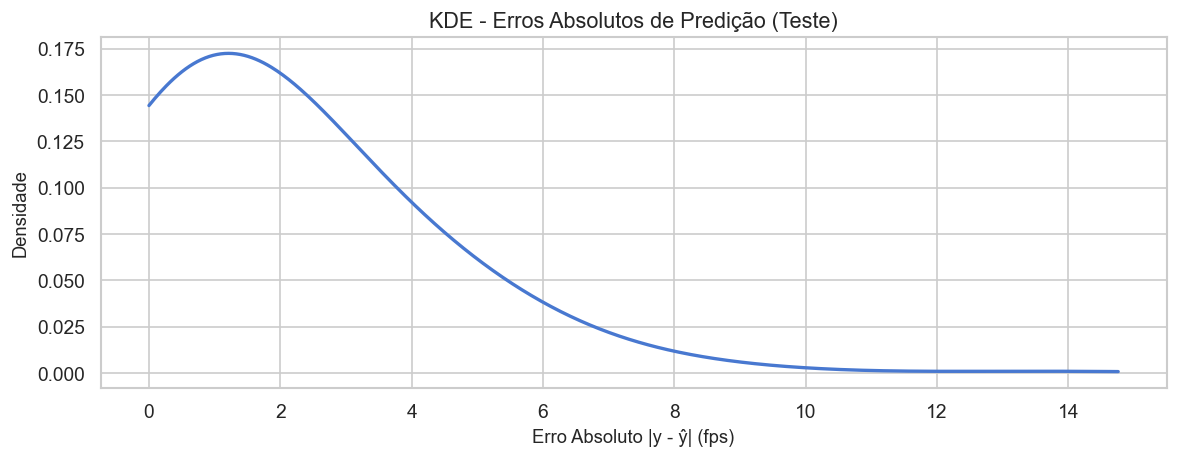
\includegraphics[width=0.8\textwidth]{figuras/fig_kde_errors.png}
\caption{KDE dos erros absolutos de predição no conjunto de teste.}
\label{fig:kde_errors}
\end{figure}

A Figura~\ref{fig:kde_errors} mostra que os erros absolutos concentram-se principalmente entre 0 e 4 fps, com pico próximo de 1 fps. A distribuição, entretanto, apresenta uma assimetria à direita e uma cauda que alcança aproximadamente 14 fps, indicando a ocorrência de alguns erros maiores. Esses casos podem estar relacionados à distribuição bimodal observada na Figura~\ref{fig:kde_framerate}, na qual o sistema alterna entre dois regimes distintos de operação, sugerindo que os maiores erros tendem a ocorrer nos momentos de transição entre esses regimes.

\subsubsection{Discussão da Acurácia}

O modelo linear atingiu NMAE de 10{,}39\%, valor inferior ao limite de 15\% estabelecido no projeto, indicando boa capacidade de predição do \emph{frame rate}. Entretanto, essa métrica representa um erro médio e não evidencia diferenças de desempenho ao longo de toda a série temporal. As análises apresentadas anteriormente mostram que o modelo reproduz adequadamente os dois regimes predominantes de operação, mas encontra maior dificuldade nos momentos de transição entre eles. Esse comportamento é consistente com a distribuição bimodal observada para o \emph{frame rate} e ajuda a explicar a presença de erros mais elevados em uma pequena parcela das observações. Além disso, os coeficientes obtidos sugerem que variáveis relacionadas à utilização de CPU, memória, carga do sistema e número de conexões TCP exercem maior influência sobre as predições. Como a regressão linear assume relações aditivas entre as variáveis, parte da dinâmica do sistema pode não ser completamente capturada, especialmente em situações de mudança abrupta de regime.


\subsection{Relação entre Tamanho do Treino, Acurácia e Tempo de Treinamento}

Para investigar o efeito do tamanho do conjunto de treino, cinco subconjuntos de tamanhos $n \in \{50, 500, 1000, 1500, 2520\}$ foram amostrados aleatoriamente (com semente fixa) a partir do conjunto de treino original de 2520 observações, gerando cinco modelos $M_1, \ldots, M_5$.

\subsubsection{Coeficientes dos Modelos}

A Tabela~\ref{tab:coefs_sizes} apresenta os coeficientes de cada um dos cinco modelos.

\begin{table}[H]
\centering
\caption{Coeficientes dos modelos lineares para diferentes tamanhos de treinamento.}
\label{tab:coefs_sizes}
\small
\begin{tabular}{lrrrrr}
\toprule
\textbf{Parâmetro} & \textbf{$n=50$} & \textbf{$n=500$} & \textbf{$n=1000$} & \textbf{$n=1500$} & \textbf{$n=2520$} \\
\midrule
Intercepto              & 36.8386 & 45.0330 & 52.2503 & 49.7976 & 49.6878 \\
cpu.idle                & -0.0383 & -0.1004 & -0.0789 & -0.0884 & -0.0921 \\
mem.used                &  0.0263 & -0.0611 & -0.1006 & -0.0790 & -0.0868 \\
proc.creation.rate      & -0.0497 & -0.0336 & -0.0183 & -0.0114 & -0.0120 \\
ctx.switch.rate         & -0.0000 & -0.0001 & -0.0001 & -0.0001 & -0.0001 \\
file.handles            & -0.0066 & -0.0025 & -0.0044 & -0.0037 & -0.0031 \\
interrupt.rate          &  0.0001 &  0.0000 &  0.0001 &  0.0000 &  0.0000 \\
load.avg.1min           & -0.0444 & -0.0711 & -0.0593 & -0.0565 & -0.0606 \\
tcp.sockets             & -0.0441 & -0.0392 & -0.0609 & -0.0698 & -0.0653 \\
pg.free.rate            &  0.0000 & -0.0000 & -0.0000 & -0.0000 & -0.0000 \\
\bottomrule
\end{tabular}
\end{table}

Com apenas 50 observações para estimar 10 parâmetros, o modelo $M_1$ apresenta instabilidade e um coeficiente inconsistente: \texttt{mem.used} assume sinal positivo ($+0{,}0263$). Isso sugeriria erroneamente que o maior uso de memória aumenta o \emph{frame rate}, o que contraria a lógica do sistema e reflete um claro \emph{overfitting} ao ruído amostral devido à escassez de dados. A partir do modelo $M_2$, com 500 amostras, os sinais dos coeficientes se estabilizam em valores negativos ou próximos de zero, e o intercepto converge para a faixa entre 49 e 52. Esse comportamento se mantém essencialmente constante nos modelos seguintes, de 1000 a 2520 amostras.

\subsubsection{Tempo de Treinamento e NMAE}

A Tabela~\ref{tab:nmae_time} sintetiza o tempo de treinamento (em milissegundos) e o NMAE no conjunto de teste para cada um dos cinco modelos.

\begin{table}[H]
\centering
\caption{NMAE e tempo de treinamento dos modelos lineares.}
\label{tab:nmae_time}
\begin{tabular}{lrrr}
\toprule
\textbf{Modelo} & \textbf{$n$ (treino)} & \textbf{Tempo (ms)} & \textbf{NMAE (\%)} \\
\midrule
$M_1$ & 50   & 0.7732 & 11.5182 \\
$M_2$ & 500  & 0.5827 & 10.5750 \\
$M_3$ & 1000 & 0.6847 & 10.4925 \\
$M_4$ & 1500 & 0.7412 & 10.3776 \\
$M_5$ & 2520 & 0.8030 & 10.3877 \\
\bottomrule
\end{tabular}
\end{table}

Todos os cinco modelos avaliados ficaram abaixo do limite de 15\% para o NMAE, exibindo uma dinâmica clara de convergência. A redução de erro mais expressiva ocorre entre 50 e 500 observações, intervalo em que o NMAE cai de 11{,}52\% para 10{,}58\%, coincidindo com o período em que os coeficientes ganham estabilidade. A partir de 500 amostras, os ganhos tornam-se marginais, com uma melhoria de apenas 0{,}19 ponto percentual até atingir o modelo completo com 2520 observações, onde o erro estabiliza em torno de 10{,}4\%. Esse comportamento indica que a limitação principal não reside no volume de dados, mas no viés da própria abordagem linear. A bimodalidade do \emph{frame rate} introduz uma não linearidade estrutural que uma regressão linear é incapaz de capturar, independentemente da quantidade de dados oferecida no treinamento.

\begin{figure}[H]
\centering
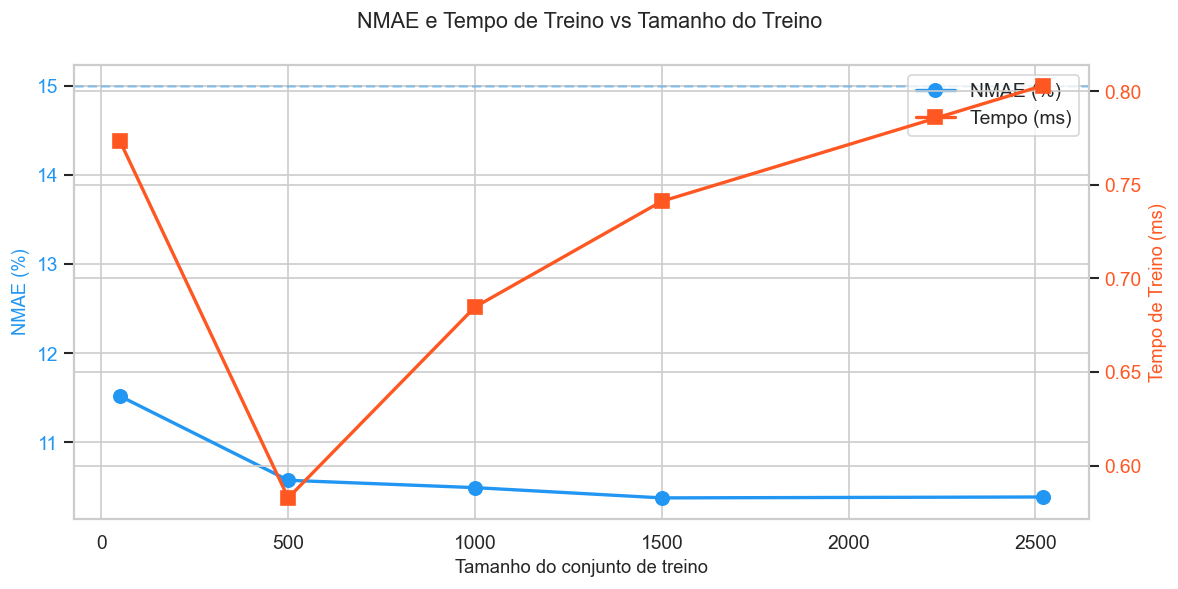
\includegraphics[width=0.85\textwidth]{figuras/fig_nmae_time_traintest.png}
\caption{NMAE e tempo de treinamento em função do tamanho do conjunto de treino.}
\label{fig:nmae_time}
\end{figure}

Sob a perspectiva computacional, a solução analítica dos Mínimos Quadrados Ordinários possui complexidade teórica $O\left(np^2 + p^3\right)$. Com o número de variáveis preditoras fixado em $p=9$, seria esperado um crescimento linear do tempo de execução em função de $n$. Contudo, na prática, todos os tempos mensurados ficaram abaixo de 1 milissegundo e sem uma tendência monotônica clara, ocorrendo situações em que treinos com bases maiores foram concluídos mais rapidamente do que com bases menores. Nessa escala de dados, o tempo real de processamento é da ordem de microssegundos, sendo amplamente dominado por \emph{overheads} fixos do ambiente, como alocação de memória, chamadas às rotinas internas do \texttt{NumPy} e o próprio escalonamento do sistema operacional. Assim, para o volume de dados considerado neste trabalho, o tamanho do conjunto de treinamento tem impacto praticamente nulo sobre o custo computacional, mas influencia diretamente a estabilidade dos parâmetros estimados e a qualidade das predições.

\section{Task III - Estimação de Conformidade e Violação do SLA a partir das Estatísticas de Dispositivo}
\label{sec:taskIII}


\subsection{Transformação do Problema em Classificação Binária}

Na Task III, a variável contínua \texttt{frame.rate} foi convertida em uma variável binária com base no critério de SLA adotado no projeto. Observações com \texttt{frame.rate} maior ou igual a 18 fps foram classificadas como conformes ao SLA, enquanto observações abaixo desse valor foram classificadas como violações. Formalmente, define-se o rótulo binário como:

\begin{equation}
    y_{SLA} =
    \begin{cases}
    1, & \text{se } \texttt{frame.rate} \geq 18,\\
    0, & \text{se } \texttt{frame.rate} < 18.
    \end{cases}
\end{equation}

A definição apresentada anteriormente foi implementada diretamente no código:

\begin{lstlisting}
y_bin = (df['frame.rate'].values >= 18).astype(int)
\end{lstlisting}

A regressão logística foi utilizada para estimar a probabilidade de conformidade do SLA a partir das estatísticas do servidor, modelando:

\begin{equation}
    P(y=1\mid X)=\sigma(\theta_0+\boldsymbol{\theta}^T\mathbf{x})
    =\frac{1}{1+e^{-(\theta_0+\boldsymbol{\theta}^T\mathbf{x})}},
\end{equation}

em que $\sigma(\cdot)$ representa a função sigmoide. A mesma divisão treino/teste utilizada na Task II foi mantida, com 2520 observações para treinamento (70\%) e 1080 para teste (30\%). As proporções de conformidade foram de 52{,}14\% no conjunto de treinamento e 50{,}46\% no conjunto de teste, caracterizando uma distribuição relativamente equilibrada entre as duas classes.


\subsection{Impacto do Tamanho do Conjunto de Treinamento no Desempenho do Modelo}

Como na Task~II, cinco classificadores $C_1, \ldots, C_5$ foram treinados sobre subconjuntos de tamanho $n \in \{50, 500, 1000, 1500, 2520\}$, com \texttt{LogisticRegression(max\_iter=10\,000)} do \texttt{scikit-learn} para garantir convergência mesmo nos modelos que exigem mais iterações.

\subsubsection{Coeficientes dos Classificadores}

A Tabela~\ref{tab:coefs_clf} apresenta os coeficientes de cada um dos cinco classificadores.

\begin{table}[H]
\centering
\caption{Coeficientes dos classificadores $C_1$ a $C_5$, por tamanho do conjunto de treino.}
\label{tab:coefs_clf}
\small
\begin{tabular}{lrrrrr}
\toprule
\textbf{Parâmetro} & \textbf{$n=50$} & \textbf{$n=500$} & \textbf{$n=1000$} & \textbf{$n=1500$} & \textbf{$n=2520$} \\
\midrule
Intercepto              & -0.0024 &  0.0010 &  0.0014 & 25.4995 & 23.6270 \\
cpu.idle                &  0.0016 & -0.0795 & -0.0164 & -0.0790 & -0.0976 \\
mem.used                &  0.6292 & -0.0321 & -0.0562 & -0.1060 & -0.1036 \\
proc.creation.rate      & -0.2935 & -0.0740 & -0.0384 & -0.0163 & -0.0079 \\
ctx.switch.rate         & -0.0012 & -0.0000 &  0.0000 & -0.0001 & -0.0001 \\
file.handles            & -0.0448 &  0.0037 &  0.0020 & -0.0025 & -0.0015 \\
interrupt.rate          &  0.0067 &  0.0004 &  0.0006 &  0.0001 &  0.0002 \\
load.avg.1min           & -0.3877 & -0.0864 & -0.0896 & -0.0550 & -0.0582 \\
tcp.sockets             &  0.5639 & -0.0593 & -0.0780 & -0.0590 & -0.0651 \\
pg.free.rate            &  0.0005 & -0.0000 & -0.0000 & -0.0000 & -0.0000 \\
\bottomrule
\end{tabular}
\end{table}

Com apenas 50 observações, o modelo apresenta maior variabilidade nos coeficientes estimados. Em particular, \texttt{mem.used} e \texttt{tcp.sockets} assumem coeficientes positivos, diferentemente do observado nos demais modelos. À medida que o tamanho do conjunto de treinamento aumenta, os coeficientes tornam-se mais estáveis e passam a indicar uma relação mais consistente entre o aumento da carga do sistema e a redução da probabilidade de conformidade com o SLA. O intercepto também converge para valores semelhantes nos modelos treinados com 1500 e 2520 observações, sugerindo maior estabilidade da fronteira de decisão.

\subsubsection{Tempo de Treinamento e Erro de Classificação (ERR)}

O desempenho dos classificadores foi avaliado por meio da métrica \emph{Classification Error} (ERR), definida:

\begin{equation}
\mathrm{ERR} = 1 - \frac{TP + TN}{m},
\label{eq:err}
\end{equation}

Essa métrica é equivalente a $1-\text{acurácia}$, sendo considerado satisfatório um classificador com $\mathrm{ERR}<15\%$, conforme estabelecido no projeto. Como o conjunto de teste contém $m=1080$ observações, o cálculo do erro de classificação foi realizado com base nesse total. A Tabela~\ref{tab:err_time} reúne os resultados obtidos para cada modelo, incluindo tempo de treinamento, acurácia, ERR e os componentes da matriz de confusão (TP, TN, FP e FN). Neste contexto, TP representa observações corretamente classificadas como conformes ao SLA, enquanto TN representa observações corretamente classificadas como violações.


\begin{table}[H]
\centering
\caption{Tempo de treinamento, acurácia, ERR e matriz de confusão para diferentes tamanhos do conjunto de treinamento.}
\label{tab:err_time}
\scriptsize
\setlength{\tabcolsep}{4pt}
\begin{tabular}{rrrrrrrr}
\toprule
\textbf{$n$} & \textbf{Tempo (ms)} & \textbf{Acurácia} & \textbf{ERR (\%)} & \textbf{TP} & \textbf{TN} & \textbf{FP} & \textbf{FN} \\
\midrule
50   & 69.21   & 0.8463 & 15.3704 & 438 & 476 & 59 & 107 \\
500  & 251.82  & 0.8704 & 12.9630 & 465 & 475 & 60 & 80 \\
1000 & 212.73  & 0.8713 & 12.8704 & 464 & 477 & 58 & 81 \\
1500 & 1322.96 & 0.8861 & 11.3889 & 479 & 478 & 57 & 66 \\
2520 & 1979.10 & 0.8889 & 11.1111 & 486 & 474 & 61 & 59 \\
\bottomrule
\end{tabular}
\end{table}

O classificador treinado com apenas 50 observações foi o único que não atingiu o critério de desempenho estabelecido no projeto, apresentando ERR de 15{,}37\%. A partir de 500 observações, todos os modelos passaram a satisfazer o limite de 15\%, com melhoria gradual até o modelo treinado com o conjunto completo, que obteve ERR de 11{,}11\% e acurácia de 88{,}89\%.

\begin{figure}[H]
\centering
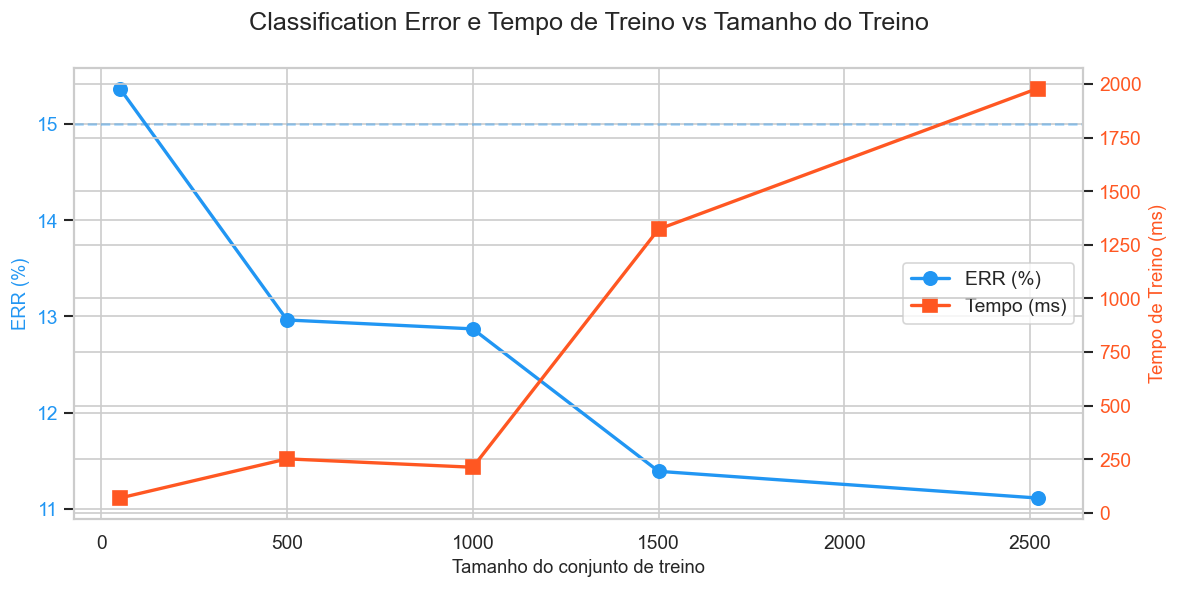
\includegraphics[width=0.85\textwidth]{figuras/fig_err_time_traintest.png}
\caption{Erro de classificação e tempo de treinamento em função do tamanho do conjunto de treino.}
\label{fig:err_time}
\end{figure}

A análise da matriz de confusão mostra que os falsos positivos permanecem relativamente estáveis entre os modelos, variando entre 57 e 61 observações. A principal melhoria ocorre na redução dos falsos negativos, que diminuem de 107 para 59 à medida que o tamanho do conjunto de treinamento aumenta. Isso indica que os ganhos obtidos com mais dados estão associados principalmente à maior capacidade do classificador em identificar corretamente observações conformes ao SLA que anteriormente eram classificadas como violações.

A Figura~\ref{fig:err_time} mostra que o ERR continua diminuindo mesmo após 1000 observações, diferentemente do comportamento observado na regressão linear, cujo erro se estabilizou mais rapidamente. Ao mesmo tempo, o tempo de treinamento cresce de forma significativa para os modelos com 1500 e 2520 observações. Ainda assim, o ganho em desempenho permanece perceptível, indicando que a regressão logística continua se beneficiando do aumento do conjunto de treinamento na definição da fronteira de decisão entre conformidade e violação do SLA.

\subsubsection{Número de Iterações}

A Tabela~\ref{tab:iteracoes} apresenta, para cada tamanho do conjunto de treinamento, o erro de classificação (ERR), o tempo de treinamento e o número de iterações necessárias para a convergência do algoritmo L-BFGS utilizado pela regressão logística.

\begin{table}[H]
\centering
\caption{ERR, tempo e número de iterações da regressão logística.}
\label{tab:iteracoes}
\begin{tabular}{rrrr}
\toprule
\textbf{$n$} & \textbf{ERR} (\%) & \textbf{Tempo (ms)} & \textbf{Iterações} \\
\midrule
50 & 15,37 & 69,21 & 344 \\
500 & 12,96 & 251,82 & 1249 \\
1000 & 12,87 & 212,73 & 988 \\
1500 & 11,39 & 1322,96 & 5404 \\
2520 & 11,11 & 1979,10 & 6872 \\
\bottomrule
\end{tabular}
\end{table}

Diferentemente da regressão linear, cujo treinamento foi concluído em menos de 1 ms para todos os experimentos, a regressão logística apresentou tempos significativamente maiores e mais sensíveis ao tamanho do conjunto de treinamento. Como o treinamento é realizado por um processo iterativo de otimização, o tempo total depende não apenas da quantidade de observações, mas também do número de iterações necessárias para atingir a convergência.

Esse comportamento pode ser observado ao comparar os modelos treinados com 500 e 1000 observações. Embora o segundo utilize mais dados, seu tempo de treinamento foi menor (212,73 ms contra 251,82 ms), pois convergiu em menos iterações (988 contra 1249). Já os modelos treinados com 1500 e 2520 observações exigiram 5404 e 6872 iterações, respectivamente, resultando em um aumento expressivo do tempo de execução.

Em termos de desempenho, observa-se uma redução gradual do ERR à medida que o conjunto de treinamento aumenta, passando de 15{,}37\% para 11{,}11\%. Assim, embora conjuntos maiores demandem mais tempo para convergência, eles também produzem classificadores mais precisos. Os resultados indicam que a relação entre tamanho do conjunto de treinamento e tempo de execução não é estritamente linear, uma vez que o comportamento do processo de otimização influencia diretamente o número de iterações necessárias para a convergência.

\subsection{Análise do Melhor Classificador}

O melhor classificador foi o $C_5$, treinado com 2520 observações, apresentando ERR de $=11{,}11\%$. A Figura~\ref{fig:scatter} mostra o comportamento desse classificador ao longo da sequência temporal original do conjunto de teste, indicando para cada observação se a decisão tomada foi correta ou incorreta.

\begin{figure}[H]
\centering
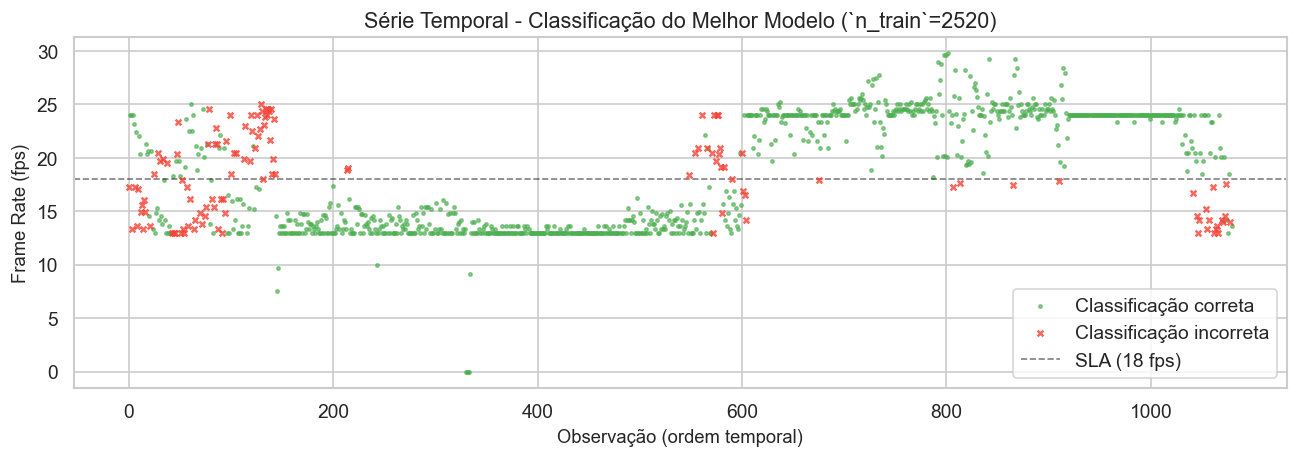
\includegraphics[width=0.95\textwidth]{figuras/fig_classification_scatter.png}
\caption{Série temporal do \emph{frame rate} com acertos e erros do melhor classificador.}
\label{fig:scatter}
\end{figure}

A Figura~\ref{fig:scatter} mostra que a maioria dos erros ocorre quando o \emph{frame rate} está próximo do limiar de SLA de 18 fps. Em contrapartida, observações com valores mais distantes desse limite, tanto na região próxima de 13 fps quanto na região próxima de 24 fps, são classificadas corretamente na maior parte dos casos. Esse resultado ajuda a explicar por que o classificador apresenta bom desempenho global, apesar dos erros observados em pontos específicos.

Também é possível notar que os erros não aparecem distribuídos de forma uniforme ao longo da série. Há uma concentração maior nas primeiras 200 observações e novamente por volta das observações 500 a 600. Já entre aproximadamente 300 e 500 observações, bem como entre 800 e 1000, predominam classificações corretas. Visualmente, esses erros parecem ocorrer em trechos nos quais o sistema alterna entre níveis distintos de desempenho, enquanto os acertos se concentram em períodos mais estáveis.

\subsection{Relação entre Tamanho do Treino e Acurácia dos Classificadores} 

A Tabela~\ref{tab:err_accuracy} apresenta os valores de ERR e acurácia obtidos para diferentes tamanhos do conjunto de treinamento.

\begin{table}[H]
\centering
\caption{ERR e acurácia dos classificadores.}
\label{tab:err_accuracy}
\begin{tabular}{rrr}
\toprule
\textbf{$n$} & \textbf{ERR (\%)} & \textbf{Acurácia (\%)} \\
\midrule
50   & 15.37 & 84.63 \\
500  & 12.96 & 87.04 \\
1000 & 12.87 & 87.13 \\
1500 & 11.39 & 88.61 \\
2520 & 11.11 & 88.89 \\
\bottomrule
\end{tabular}
\end{table}

O aumento do conjunto de treinamento produz uma redução gradual do erro de classificação. O modelo treinado com apenas 50 observações foi o único que não atingiu o critério estabelecido no projeto, apresentando ERR de 15{,}37\%. Esse resultado é consistente com a maior instabilidade observada nos coeficientes desse classificador. A partir de 500 observações, todos os modelos passaram a apresentar ERR inferior a 15\%, com melhoria contínua até o modelo treinado com o conjunto completo, que alcançou ERR de 11{,}11\% e acurácia de 88,89%.

Diferentemente do observado na Task II, em que o NMAE da regressão linear se estabilizou rapidamente, a regressão logística continuou apresentando ganhos de desempenho à medida que novas observações foram incorporadas ao treinamento. Ainda assim, a redução do erro torna-se progressivamente menor para conjuntos maiores, sugerindo convergência em torno de 11\%. Esse resultado indica que o aumento da quantidade de dados melhora a capacidade de classificação do modelo, mas não elimina completamente os erros associados às observações próximas ao limiar de SLA, que representam os casos mais difíceis de distinguir.

\subsection{Relação entre Tamanho do Treino e Tempo de Treinamento} 

A Tabela~\ref{tab:iteracoes} apresenta o ERR, o tempo de treinamento e o número de iterações necessárias para a convergência da regressão logística em cada tamanho de conjunto de treinamento.

Diferentemente da regressão linear analisada na Task II, cujos modelos foram treinados em menos de 1 ms, a regressão logística apresentou tempos significativamente maiores, variando de 69 ms a aproximadamente 2 s. Essa diferença é consequência do processo iterativo de otimização utilizado para estimar os parâmetros do modelo, em contraste com a solução analítica empregada pela regressão linear.

Observa-se que o tempo de treinamento não depende apenas da quantidade de observações, mas também do número de iterações necessárias para a convergência. Isso explica, por exemplo, por que o modelo treinado com 1000 observações foi mais rápido que o modelo treinado com 500 observações: embora possuísse mais dados, convergiu em menos iterações (988 contra 1249). Por outro lado, os modelos treinados com 1500 e 2520 observações exigiram 5404 e 6872 iterações, respectivamente, resultando em um aumento expressivo do tempo de execução.

Durante os experimentos, o parâmetro \texttt{max.iter} precisou ser aumentado para permitir a convergência dos modelos maiores, uma vez que os valores padrão não seriam suficientes para completar o processo de otimização. Apesar do crescimento observado, os tempos obtidos permanecem compatíveis com cenários de análise exploratória e monitoramento offline, especialmente quando comparados ao ganho de desempenho alcançado pelos classificadores treinados com conjuntos maiores.


\section{Conclusão}
\label{sec:conclusao}

Este trabalho investigou a utilização de estatísticas de sistema operacional para estimar a qualidade de serviço de uma aplicação de vídeo sob demanda e sua conformidade com um SLA baseado em \emph{frame rate}. Os resultados mostraram que informações coletadas exclusivamente no lado do servidor são capazes de fornecer estimativas úteis tanto para a predição do \emph{frame rate} quanto para a detecção de violações de SLA.

Na Task I, a análise exploratória revelou características importantes do ambiente monitorado, destacando a elevada utilização dos recursos do servidor e a distribuição bimodal da taxa de quadros. Essa característica mostrou-se particularmente relevante para a interpretação dos resultados obtidos nas etapas posteriores.

Na Task II, a regressão linear atingiu NMAE de 10{,}39\%, valor inferior ao limite de 15\% estabelecido no projeto. O modelo foi capaz de capturar adequadamente a tendência geral do \emph{frame rate}, embora os maiores erros tenham se concentrado nas regiões de transição entre os dois regimes de operação observados nos dados. Além disso, verificou-se que o erro estabiliza rapidamente com o aumento do conjunto de treinamento, enquanto o tempo de treinamento permanece praticamente desprezível para a escala de dados considerada.

Na Task III, a regressão logística obteve ERR de 11{,}11\%, também satisfazendo o critério de desempenho definido no enunciado. Assim como observado na regressão linear, os erros de classificação concentraram-se principalmente nas proximidades do limiar de SLA, região em que a distinção entre conformidade e violação se torna mais difícil. O aumento do conjunto de treinamento contribuiu para a redução do erro e para a estabilização dos coeficientes do modelo, embora com um custo computacional significativamente superior ao observado na regressão linear.

De forma geral, os resultados indicam que modelos lineares e logísticos constituem soluções simples, interpretáveis e eficazes para a estimação de métricas de serviço e monitoramento de conformidade com SLA. Entretanto, a presença de dois regimes distintos de operação e a concentração dos erros nas regiões de transição sugerem que modelos não lineares podem representar uma alternativa promissora para trabalhos futuros, com potencial para capturar relações mais complexas entre as estatísticas do dispositivo e a qualidade percebida do serviço.


\section{Atividade Opcional - Desafio dos Datasets 5G}
\label{sec:opcional}

Além das tarefas obrigatórias descritas nas seções anteriores, foi desenvolvida a atividade opcional \emph{5G Dataset Challenge}. O enunciado propõe quatro atividades independentes (A, B, C e D), todas elas exploradas neste trabalho.

\subsection{Conjuntos de Dados Utilizados}
\label{sec:opcional-dados}

Os experimentos utilizam três conjuntos de dados do repositório \texttt{intrig-unicamp/hackathon5G}, coletados em campo com um \emph{smartphone} 5G na cidade de São Paulo. A Tabela~\ref{tab:opcional-datasets} resume cada um deles. Ao todo, foram carregados 34.281 registros de rede móvel, distribuídos em 13 arquivos de sessão.

\begin{table}[H]
\centering
\caption{Conjuntos de dados utilizados na atividade opcional.}
\label{tab:opcional-datasets}
\begin{tabular}{lp{6.2cm}p{4.8cm}}
\toprule
\textbf{Dataset} & \textbf{Descrição} & \textbf{Uso neste trabalho} \\
\midrule
\texttt{g-nettrack-pro} & Métricas de rede móvel (RSRP, RSRQ, SNR, CQI, tecnologia, coordenadas, célula servidora) coletadas em 13 sessões (a pé, de carro, metrô e indoor) & Atividades A, B e D \\
\texttt{mosaico} (Anatel) & Cadastro de Estações Rádio Base licenciadas no Brasil (localização, tecnologia, frequência, azimute, potência) & Atividades A, C e D \\
\texttt{youtube-qoe} & Métricas de \emph{streaming} de vídeo do YouTube (resolução, saúde do \emph{buffer}, alertas de QoE), capturadas via PCAPdroid & Atividade C \\
\bottomrule
\end{tabular}
\end{table}

\subsection{Análise Exploratória dos Dados}
\label{sec:opcional-exploracao-dados}

A primeira etapa consistiu em caracterizar a base de medições de rede. A Tabela~\ref{tab:opcional-cenarios} apresenta a distribuição de registros por cenário de mobilidade, extraído a partir do nome dos arquivos, e por tecnologia de rede.

\begin{table}[H]
\centering
\caption{Distribuição dos registros do \texttt{g-nettrack-pro} por cenário e por tecnologia.}
\label{tab:opcional-cenarios}
\begin{tabular}{lrr|lrr}
\toprule
\textbf{Cenário} & \textbf{Registros} & \textbf{\%} & \textbf{Tecnologia} & \textbf{Registros} & \textbf{\%} \\
\midrule
Sessão correlacionada (QoE) & 15.862 & 46,3 & 5G & 17.099 & 49,9 \\
Pedestre                    & 10.270 & 30,0 & 4G & 16.843 & 49,1 \\
Veículo                     & 4.527  & 13,2 & 3G & 251    & 0,7 \\
Indoor                      & 2.946  & 8,6  & 2G & 35     & 0,1 \\
Metrô                       & 676    & 2,0  & Sem registro & 53 & 0,2 \\
\bottomrule
\end{tabular}
\end{table}

Observa-se que as medições concentram-se principalmente em 4G e 5G, que juntas representam a
quase totalidade dos registros. Em relação aos cenários de mobilidade, há maior volume de dados
em sessões sem rótulo direto no nome do arquivo e em trajetos de pedestre, enquanto o cenário de
metrô possui número bastante menor de amostras.

A Figura~\ref{fig:opcional-boxplots} compara as métricas de qualidade de sinal entre 4G e 5G. O RSRP e o CQI apresentam valores médios semelhantes nas duas tecnologias, indicando potência recebida e qualidade de canal próximas. As diferenças mais visíveis aparecem no RSRQ, melhor em 5G, e no SNR, maior em 4G nesta amostra. Esses resultados mostram que a comparação entre 4G e 5G depende da métrica analisada, reforçando a necessidade de avaliar conjuntamente diferentes indicadores de qualidade de sinal.

\begin{figure}[H]
\centering
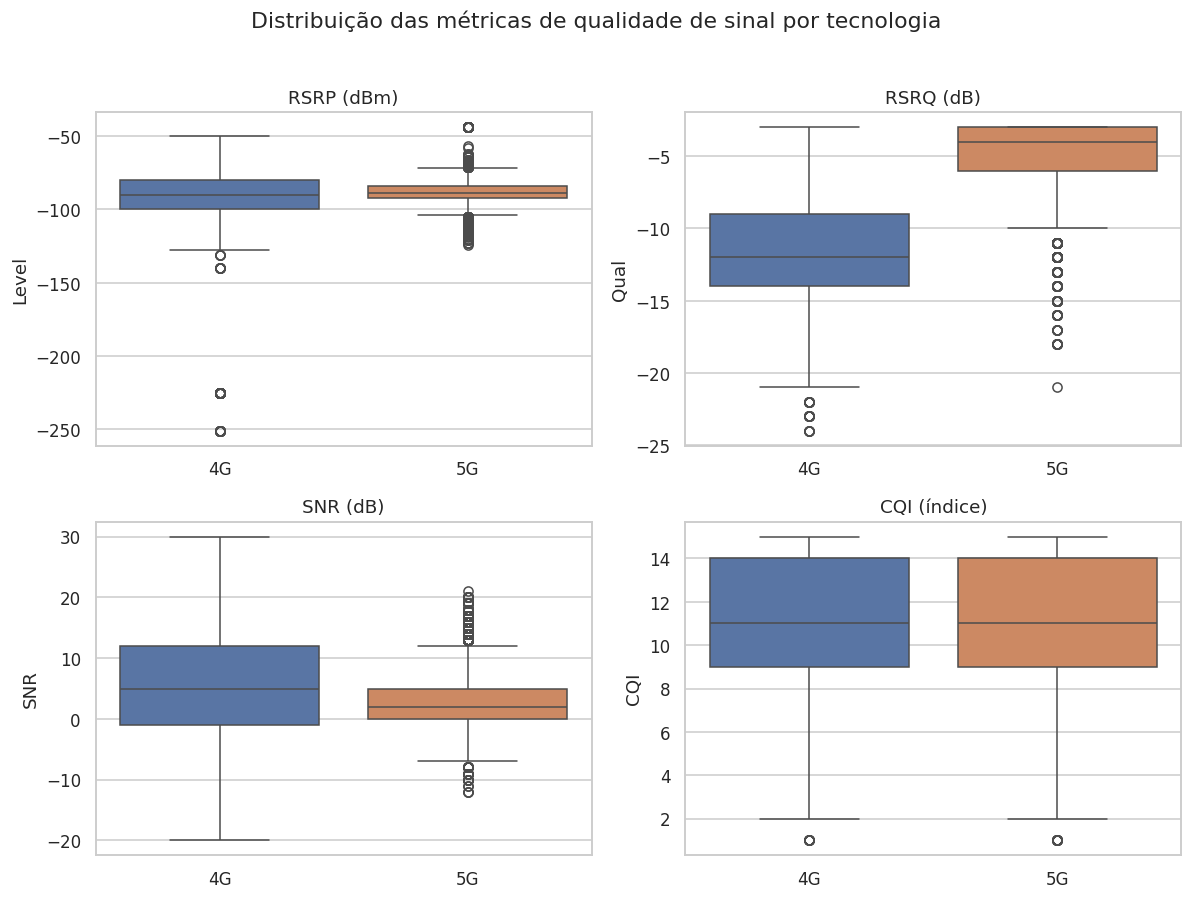
\includegraphics[width=0.85\textwidth]{figuras/fig_5g_boxplots_sinal.png}
\caption{Distribuição das métricas de qualidade de sinal por tecnologia de rede.}
\label{fig:opcional-boxplots}
\end{figure}

\begin{figure}[H]
\centering
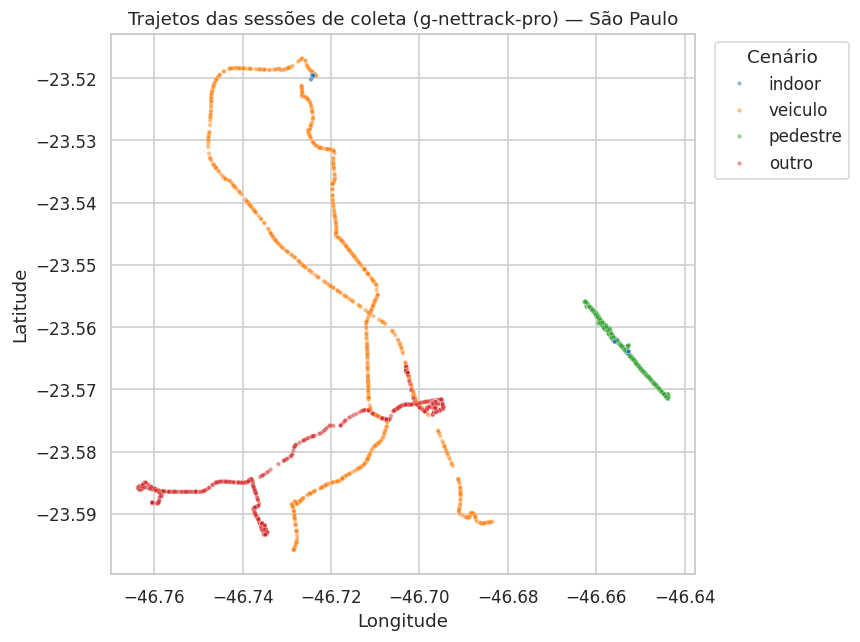
\includegraphics[width=0.75\textwidth]{figuras/fig_5g_trajetos_mapa.png}
\caption{Trajetos das sessões de coleta do G-NetTrack Pro em São Paulo.}
\label{fig:opcional-trajetos}
\end{figure}

A Figura~\ref{fig:opcional-trajetos} apresenta os trajetos de coleta realizados na cidade de São Paulo. Observa-se que a maior parte das sessões se concentra em regiões específicas, especialmente no entorno da Avenida Paulista, enquanto uma sessão realizada de carro cobre uma área mais ampla. A proximidade entre pontos consecutivos também evidencia a dependência espacial dos dados, aspecto importante para a interpretação das medições de sinal e mobilidade.

Para enriquecer a análise com informações de infraestrutura, os dados do Mosaico/Anatel foram recortados para a mesma região geográfica das sessões de coleta, delimitada por latitudes entre $-23{,}6258$ e $-23{,}4868$ e longitudes entre $-46{,}7937$ e $-46{,}6135$. Nesse recorte, foram encontradas 435.561 antenas licenciadas, depois agrupadas em 5.759 \emph{sites} físicos distintos a partir de coordenadas coincidentes. A Tabela~\ref{tab:mosaico} resume as tecnologias presentes nessa área, com predominância de registros LTE, WCDMA, GSM e NR.

\begin{table}[H]
\centering
\caption{Tecnologias encontradas no Mosaico dentro da região de interesse.}
\label{tab:mosaico}
\begin{tabular}{lr}
\toprule
\textbf{Tecnologia} & \textbf{Registros} \\
\midrule
LTE   & 36855 \\
WCDMA & 22042 \\
GSM   & 10212 \\
NR    & 7629 \\
DMR   & 107 \\
VHF   & 36 \\
Outras/indefinidas & 23 \\
\bottomrule
\end{tabular}
\end{table}

A Figura~\ref{fig:opcional-mosaico} mostra como esses \emph{sites} se distribuem em relação aos pontos coletados pelo \texttt{g-nettrack}. A partir desse cruzamento, foi possível associar cada ponto de medição a características da infraestrutura ao redor, como a distância até os \emph{sites} mais próximos e a densidade de antenas na vizinhança. Essas variáveis complementam as medições obtidas diretamente pelo dispositivo e ajudam a contextualizar as variações de qualidade de sinal observadas ao longo dos trajetos.

\begin{figure}[H]
\centering
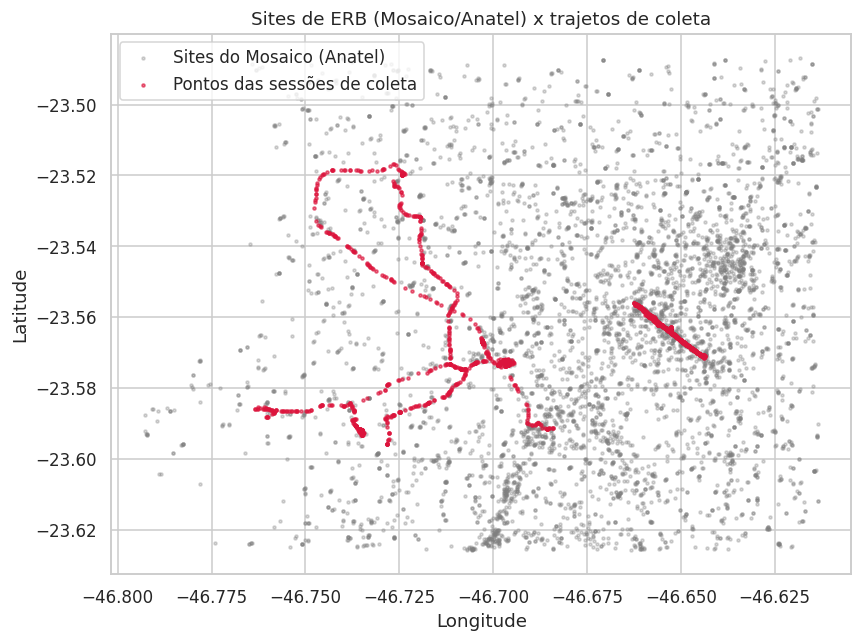
\includegraphics[width=0.75\textwidth]{figuras/fig_5g_mosaico_sites.png}
\caption{\emph{Sites} de ERB do Mosaico/Anatel (cinza) e pontos das sessões de coleta (vermelho).}
\label{fig:opcional-mosaico}
\end{figure}


\subsection{Atividade A - Predição de Qualidade de Sinal}
\label{sec:opcional-a}

A Atividade A teve como objetivo predizer um indicador de qualidade de sinal a partir das métricas coletadas no G-NetTrack Pro. O indicador escolhido foi o CQI (\emph{Channel Quality Indicator}), pois representa uma medida agregada da qualidade do canal de rádio percebida pelo aparelho. Registros 3G e 2G foram descartados, já que o CQI não é reportado de forma equivalente nesses casos. Ao final do pré-processamento, 28.983 registros 4G/5G com CQI disponível foram utilizados.

Foram comparados dois modelos de regressão Random Forest. O primeiro utilizou apenas métricas do próprio G-NetTrack, como RSRP, RSRQ, SNR, ARFCN, velocidade, tecnologia e vazão. O segundo acrescentou variáveis derivadas do Mosaico, como distância aos três sites mais próximos, número de antenas nesses sites e presença de 5G.

A Tabela~\ref{tab:opcional-A} mostra que o enriquecimento com o Mosaico melhora o desempenho do modelo. O MAE cai de 1,719 para 1,629 e o $R^2$ sobe de 0,403 para 0,460. A melhora não é suficiente para tornar a predição perfeita, mas indica que informações sobre infraestrutura próxima carregam sinal preditivo adicional em relação às métricas instantâneas do aparelho.

\begin{table}[H]
\centering
\caption{Desempenho dos modelos de regressão para o CQI (Atividade A).}
\label{tab:opcional-A}
\begin{tabular}{lrrr}
\toprule
\textbf{Modelo} & \textbf{MAE} & \textbf{RMSE} & \textbf{R\textsuperscript{2}} \\
\midrule
Sem enriquecimento (somente \texttt{g-nettrack}) & 1,719 & 2,189 & 0,403 \\
Com enriquecimento (+ Mosaico)                   & 1,629 & 2,083 & 0,460 \\
\bottomrule
\end{tabular}
\end{table}

A Figura~\ref{fig:opcional-A} mostra que as variáveis diretamente relacionadas ao canal de rádio, como SNR e nível de
sinal, permanecem entre as mais relevantes. Isso é esperado, pois o CQI é fortemente ligado à relação sinal-ruído e à qualidade instantânea do canal. As variáveis do Mosaico contribuem como informação contextual, mas não substituem as medições diretas de rede. O $R^2$ moderado também é coerente com dados de campo, nos quais fatores como interferência instantânea, carga da célula e decisões internas do dispositivo não estão completamente representados nas variáveis disponíveis.

\begin{figure}[H]
\centering
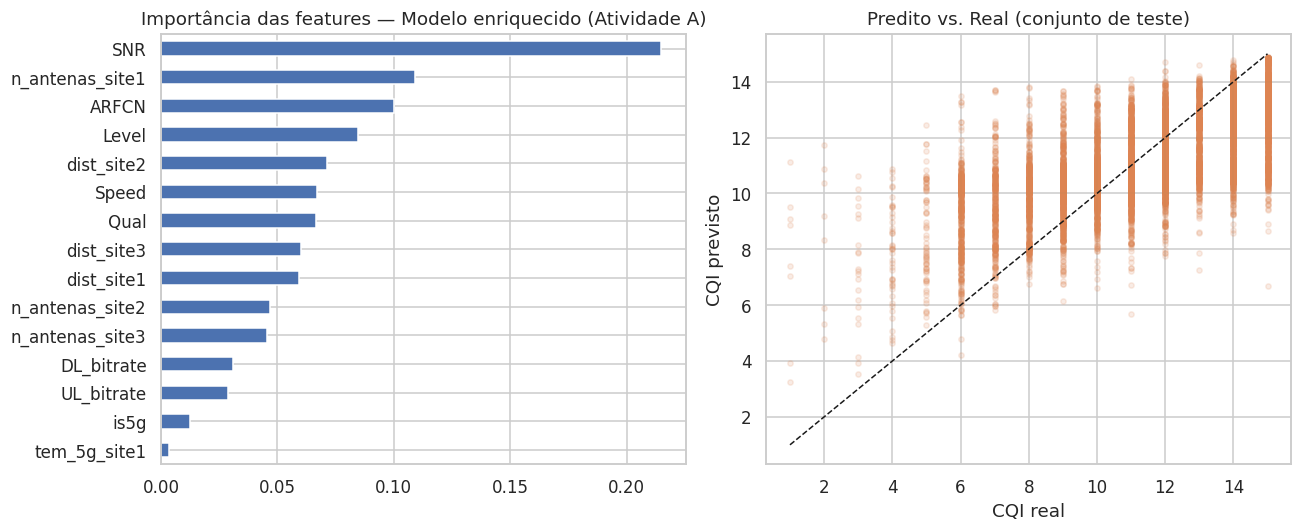
\includegraphics[width=\textwidth]{figuras/fig_5g_atividadeA.png}
\caption{Importância das variáveis no modelo enriquecido e comparação entre CQI real e previsto.}
\label{fig:opcional-A}
\end{figure}

\subsection{Atividade B - Predição do Tipo de Mobilidade}
\label{sec:opcional-b}

A Atividade B trata o problema de identificação do tipo de mobilidade como uma tarefa não supervisionada. O objetivo foi agrupar os registros sem utilizar o rótulo de cenário durante o treinamento. Para reduzir ruído de GPS e capturar padrões temporais, os registros foram agregados em janelas de 30 segundos por sessão. Para cada janela foram calculadas variáveis como velocidade média, desvio padrão da velocidade, fração de amostras sem GPS, taxa de troca de célula e fração de amostras em 5G.

Foram construídas 1.012 janelas de 30 segundos. A Tabela~\ref{tab:janelas} mostra a distribuição das janelas por cenário.

\begin{table}[H]
\centering
\caption{Distribuição das janelas de 30 segundos por cenário.}
\label{tab:janelas}
\begin{tabular}{lr}
\toprule
\textbf{Cenário} & \textbf{Janelas} \\
\midrule
outro    & 485 \\
pedestre & 311 \\
indoor   & 100 \\
veículo  & 93 \\
metrô    & 23 \\
\bottomrule
\end{tabular}
\end{table}

Como o objetivo era validar a capacidade de agrupamento em cenários conhecidos, as sessões rotuladas como ``outro'' foram removidas da avaliação quantitativa. O \emph{K-Means} foi testado para $k \in \{3,4,5,6\}$, utilizando ARI e coeficiente de silhueta como métricas. Conforme apresentado na Tabela~\ref{tab:opcional-B}, o valor $k=4$ foi escolhido por obter o melhor ARI entre os valores testados, indicando maior concordância com os rótulos reais de mobilidade. Embora a silhueta seja maior para $k=3$, esse resultado não necessariamente representa melhor aderência aos cenários de interesse, pois pode agrupar em uma mesma classe situações distintas do ponto de vista da mobilidade.

\begin{table}[H]
\centering
\caption{Resultados da clusterização para diferentes valores de k (Atividade B).}
\label{tab:opcional-B}
\begin{tabular}{rrr}
\toprule
\textbf{$k$} & \textbf{ARI} & \textbf{Silhueta} \\
\midrule
3 & 0,160 & 0,599 \\
\textbf{4} & \textbf{0,478} & 0,402 \\
5 & 0,441 & 0,435 \\
6 & 0,446 & 0,443 \\
\bottomrule
\end{tabular}
\end{table}

\begin{figure}[H]
\centering
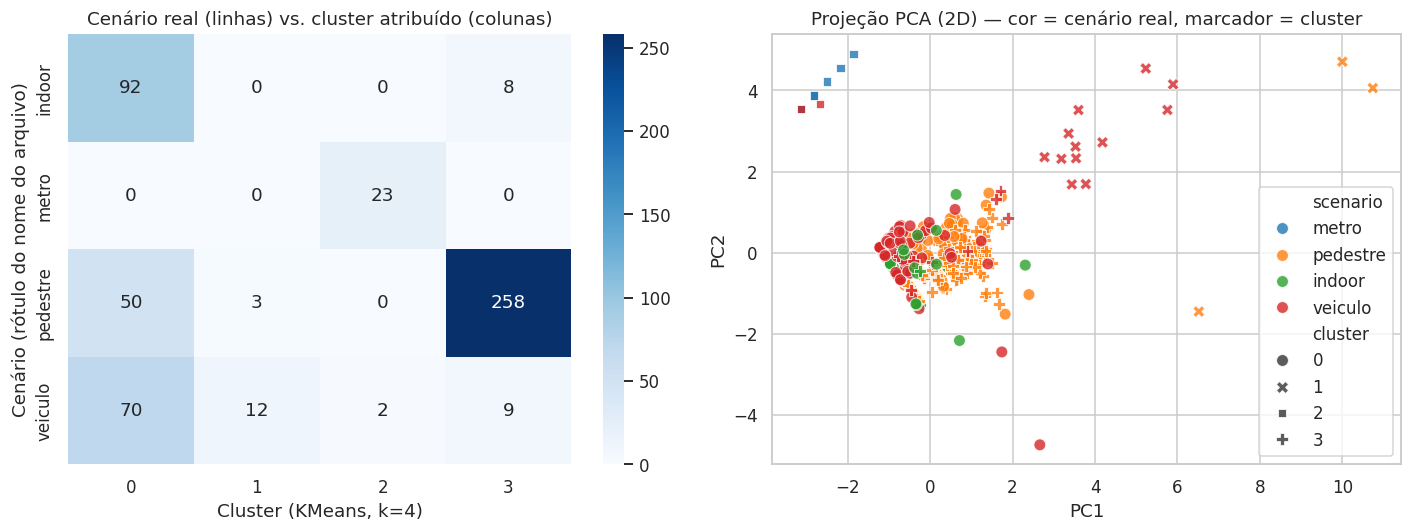
\includegraphics[width=\textwidth]{figuras/fig_5g_atividadeB.png}
\caption{Concordância entre cenário real e cluster atribuído, $k=4$ (esquerda) e projeção PCA 2D dos clusters (direita).}
\label{fig:opcional-B}
\end{figure}

A Figura~\ref{fig:opcional-B} mostra que o cenário de metrô é separado de forma bastante clara, o que é consistente
com a ausência frequente de GPS em ambiente subterrâneo e com padrões específicos de troca de célula. A separação entre pedestre e veículo também ocorre em boa parte dos casos, principalmente
devido às diferenças de velocidade. A maior confusão aparece entre indoor e trechos de veículo parado, situação esperada porque ambos podem apresentar baixa velocidade e padrões de sinal semelhantes.
Esse resultado indica que a mobilidade pode ser inferida parcialmente por variáveis simples, mas que cenários estáticos ou de baixa velocidade exigem variáveis adicionais para melhor separação.

\subsection{Atividade C - Predição de QoE de \emph{Streaming} de Vídeo}
\label{sec:opcional-c}

A Atividade C avaliou a relação entre métricas de rede móvel, localização, infraestrutura próxima e qualidade de experiência em \emph{streaming} de vídeo. A sessão de QoE utilizada foi \texttt{PCAPdroid\_24\_Feb\_16\_35\_24.pickle}, contendo 762 registros entre 16h35 e 20h35 de 24/02/2023. Essa sessão coincide temporalmente com a sessão de rede \texttt{2023-02-24\_16-35.txt}, permitindo associar os eventos de \emph{streaming} às medições de rede mais próximas no tempo.

Foi definida uma métrica contínua de QoE em escala de 1 a 5, inspirada em \emph{Mean Opinion Score} (MOS). A métrica combina qualidade de imagem, saúde do \emph{buffer}, penalização por risco de travamento, quadros descartados e alertas de QoE emitidos pelo próprio \emph{player}. A formulação utilizada é apresentada na Equação~\ref{eq:qoe}.

\begin{equation}
\text{QoE} = \text{clip}\Big(1 + 4(0,5\cdot\text{res\_score} + 0,5\cdot\text{buffer\_score}) - 1,5\cdot\text{stall} - 1,0\cdot\text{df\_score} - 1,0\cdot\text{alerta},\ [1,5]\Big)
\label{eq:qoe}
\end{equation}

A combinação entre eventos de \emph{streaming} e registros de rede foi realizado com \texttt{merge\_asof}, utilizando tolerância de 5 segundos. Todos os 762 eventos foram pareados com sucesso, correspondendo a 100\% dos registros analisados. A Tabela~\ref{tab:qoe_desc} apresenta as estatísticas descritivas da QoE estimada.

\begin{table}[H]
\centering
\caption{Estatísticas descritivas da QoE estimada.}
\label{tab:qoe_desc}
\begin{tabular}{lr}
\toprule
\textbf{Estatística} & \textbf{Valor} \\
\midrule
Registros & 762 \\
Média & 3,763 \\
Desvio padrão & 1,585 \\
Mínimo & 1,000 \\
P25 & 1,500 \\
Mediana & 5,000 \\
P75 & 5,000 \\
Máximo & 5,000 \\
\bottomrule
\end{tabular}
\end{table}

\begin{figure}[H]
\centering
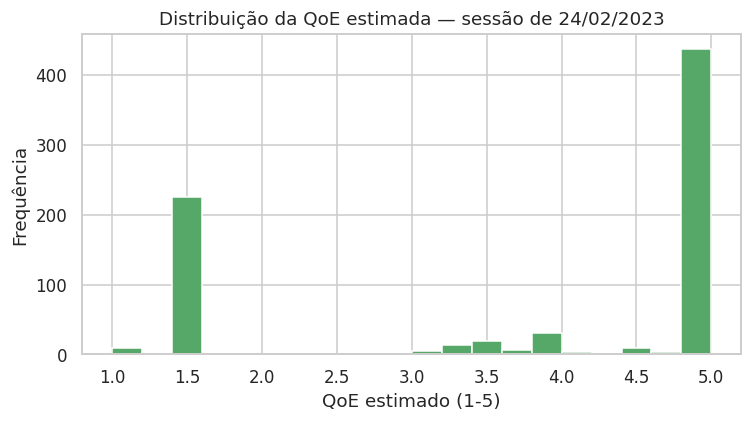
\includegraphics[width=0.70\textwidth]{figuras/fig_5g_atividadeC_hist.png}
\caption{Distribuição da QoE estimada para a sessão de \emph{streaming} analisada.}
\label{fig:qoe_hist}
\end{figure}

A Figura~\ref{fig:qoe_hist} mostra concentração expressiva de valores altos de QoE, com mediana igual a 5,0. Ainda assim, o primeiro quartil em 1,5 indica que uma parcela relevante dos eventos apresentou experiência degradada, associada a situações como \emph{buffer} baixo, resolução reduzida, quadros descartados ou alertas de QoE.

A Tabela~\ref{tab:qoe_tech} apresenta a QoE média por tecnologia de rede. Observa-se que 4G e 5G tiveram desempenho médio semelhante nesta sessão, com leve vantagem para 4G. Esse resultado não indica superioridade geral do 4G, mas sugere que, nesta coleta específica, a tecnologia nominal não foi suficiente para explicar sozinha a experiência de \emph{streaming}.

\begin{table}[H]
\centering
\caption{QoE estimada por tecnologia de rede.}
\label{tab:qoe_tech}
\begin{tabular}{lrrr}
\toprule
\textbf{Tecnologia} & \textbf{Eventos} & \textbf{Média} & \textbf{Desvio padrão} \\
\midrule
2G & 5   & 1,500 & 0,000 \\
3G & 25  & 2,416 & 1,478 \\
4G & 334 & 3,872 & 1,558 \\
5G & 398 & 3,785 & 1,568 \\
\bottomrule
\end{tabular}
\end{table}

Foram comparados dois modelos de regressão para predizer a QoE. O Modelo 1 utiliza exclusivamente variáveis de localização e infraestrutura próxima, derivadas do Mosaico/Anatel, como distância e densidade de antenas. O Modelo 2 utiliza apenas métricas instantâneas de rede do \texttt{g-nettrack}, como RSRP, RSRQ, SNR, ARFCN, tecnologia e \emph{throughput}. A Tabela~\ref{tab:qoe_modelos} e a Figura~\ref{fig:qoe_modelos} apresentam a comparação entre os modelos.

\begin{table}[H]
\centering
\caption{Comparação dos modelos de predição de QoE.}
\label{tab:qoe_modelos}
\begin{tabular}{lrrr}
\toprule
\textbf{Modelo} & \textbf{MAE} & \textbf{RMSE} & \textbf{$R^2$} \\
\midrule
Modelo 1 (localização/antenas) & 1,167 & 1,401 & 0,166 \\
Modelo 2 (métricas de rede)    & 0,774 & 1,145 & 0,398 \\
\bottomrule
\end{tabular}
\end{table}

\begin{figure}[H]
\centering
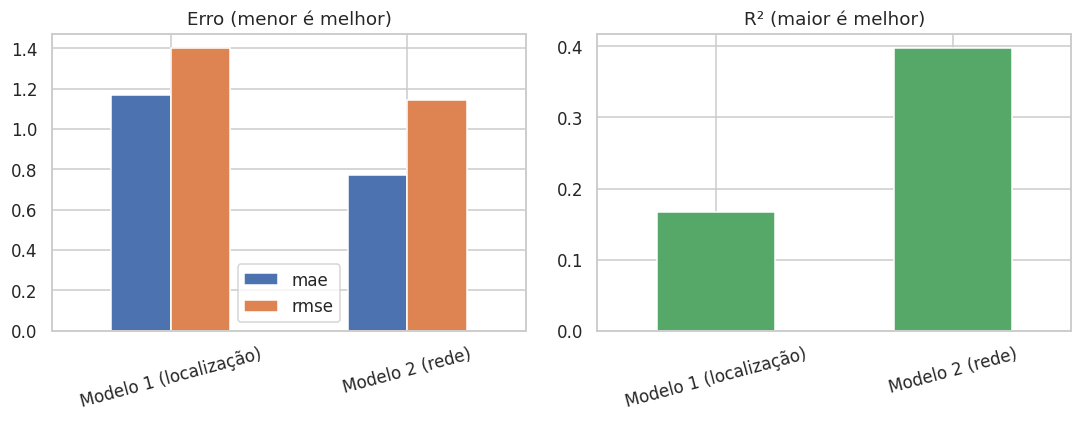
\includegraphics[width=0.82\textwidth]{figuras/fig_5g_atividadeC_comparacao.png}
\caption{Comparação de erro e capacidade explicativa entre os modelos de predição de QoE.}
\label{fig:qoe_modelos}
\end{figure}

Os resultados mostram que o Modelo 2 supera o Modelo 1 em todas as métricas avaliadas, reduzindo o MAE de 1,167 para 0,774 e elevando o $R^2$ de 0,166 para 0,398. Isso indica que a QoE de \emph{streaming} está mais diretamente associada ao estado instantâneo da conexão do que apenas à proximidade geográfica de antenas. As variáveis de localização e infraestrutura funcionam como informação contextual relevante, mas não capturam sozinhas variações momentâneas de carga, escalonamento de rádio e qualidade do canal.


\subsection{Atividade D - Inferência da Célula/Estação Base Conectada}
\label{sec:opcional-d}

A Atividade D teve como objetivo inferir a célula servidora, identificada pelo \texttt{CGI}, a partir das coordenadas do dispositivo e de informações sobre antenas próximas. Como o conjunto completo apresentava 90 células distintas e forte desbalanceamento entre classes, o experimento foi restrito às 15 células mais frequentes em registros 4G/5G. Esse recorte resultou em 25.282 registros, distribuídos em 15 classes e 12 sessões.

Cada ponto foi enriquecido com variáveis derivadas dos cinco \emph{sites} do Mosaico mais próximos, incluindo distância e densidade de antenas. Em seguida, foi treinado um classificador \emph{Random Forest}, avaliado de duas formas: divisão aleatória estratificada entre treino e teste (75\%/25\%) e \texttt{GroupKFold} por sessão. A segunda estratégia é mais rigorosa, pois mantém trajetos completos fora do treinamento e avalia a capacidade do modelo de generalizar para sessões não vistas.

\begin{table}[H]
\centering
\caption{Desempenho da inferência de célula servidora sob diferentes estratégias de avaliação.}
\label{tab:atividadeD}
\begin{tabular}{lrr}
\toprule
\textbf{Estratégia de avaliação} & \textbf{Acurácia} & \textbf{Acurácia balanceada} \\
\midrule
Divisão aleatória (75\%/25\%) & 0,935 & 0,925 \\
\texttt{GroupKFold} por sessão -- fold 1 & 0,082 & -- \\
\texttt{GroupKFold} por sessão -- fold 2 & 0,223 & -- \\
\texttt{GroupKFold} por sessão -- fold 3 & 0,372 & -- \\
\texttt{GroupKFold} por sessão -- fold 4 & 0,362 & -- \\
\texttt{GroupKFold} por sessão -- fold 5 & 0,469 & -- \\
\textbf{\texttt{GroupKFold} por sessão -- média} & \textbf{0,302} & \textbf{--} \\
\bottomrule
\end{tabular}
\end{table}

A Tabela~\ref{tab:atividadeD} mostra uma diferença expressiva entre as duas estratégias. Na divisão aleatória, o modelo atinge acurácia de 0,935 e acurácia balanceada de 0,925, indicando desempenho aparentemente elevado. No entanto, esse resultado tende a ser otimista, pois pontos próximos no tempo e no espaço podem aparecer simultaneamente nos conjuntos de treino e teste, fazendo com que o modelo reconheça padrões muito semelhantes aos já observados.

\begin{figure}[H]
\centering
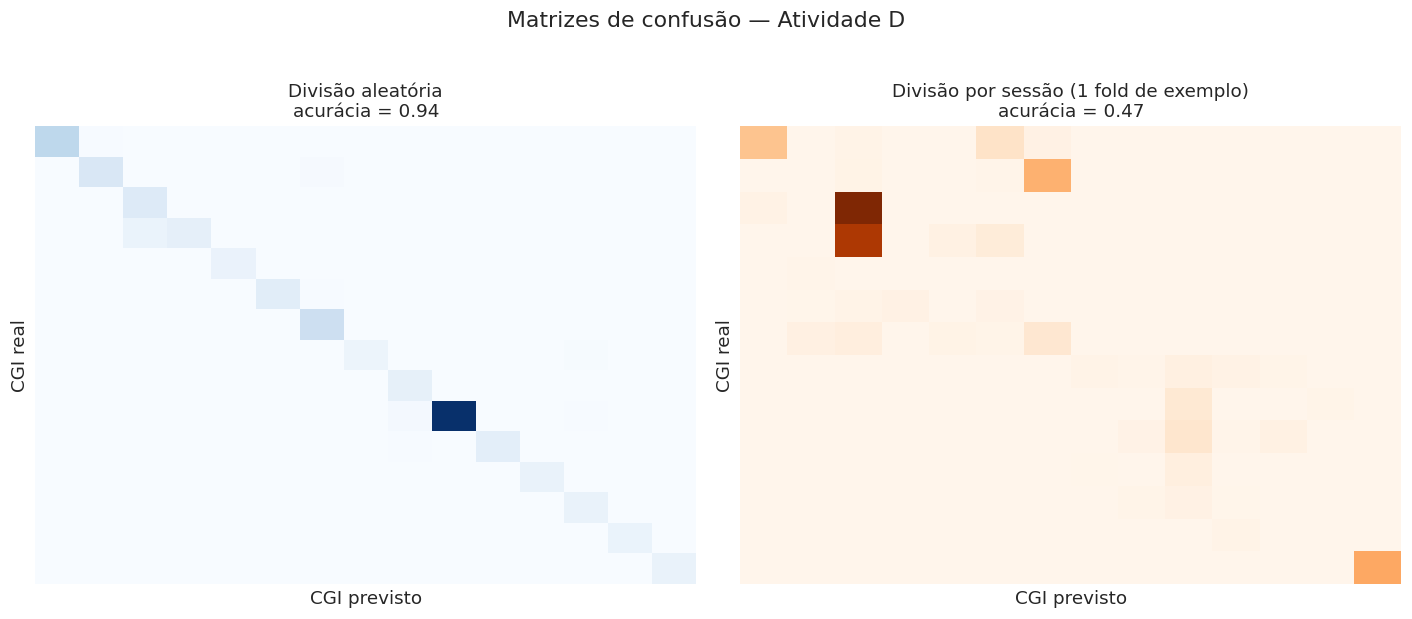
\includegraphics[width=0.95\textwidth]{figuras/fig_5g_atividadeD_confusion.png}
\caption{Matrizes de confusão para a inferência de CGI com divisão aleatória e validação por sessão.}
\label{fig:atividadeD}
\end{figure}

A avaliação por \texttt{GroupKFold} mostra um cenário mais realista. Quando sessões inteiras são mantidas fora do treinamento, a acurácia média cai para 0,302, com variação entre os folds. A Figura~\ref{fig:atividadeD} reforça esse comportamento: na divisão aleatória, a matriz de confusão apresenta maior concentração na diagonal, enquanto na validação por sessão há maior dispersão entre classes. Esse resultado revela o risco de vazamento espaço-temporal em dados de redes móveis e mostra que o modelo generaliza bem dentro de regiões já observadas, mas tem desempenho mais limitado em trajetos completamente novos.


\subsection{Síntese da Atividade Opcional}
\label{sec:opcional-conclusao}

A Tabela~\ref{tab:opcional-sintese} resume a abordagem e o principal resultado obtido em cada uma das quatro atividades.

\begin{table}[H]
\centering
\caption{Síntese das quatro atividades do desafio de \emph{datasets} 5G.}
\label{tab:opcional-sintese}
\begin{tabular}{lp{4.3cm}p{6.8cm}}
\toprule
\textbf{Atividade} & \textbf{Abordagem} & \textbf{Resultado principal} \\
\midrule
A - Qualidade de sinal & Regressão (\emph{Random Forest}) para o CQI & Enriquecimento com o Mosaico eleva o R\textsuperscript{2} de 0,403 para 0,460 \\
B - Tipo de mobilidade & Clusterização não supervisionada (\emph{K-Means}, $k=4$) & Metrô quase perfeitamente separado (ARI~$=0,478$); confusão entre indoor e veículo parado \\
C - QoE de \emph{streaming} & Função de QoE proposta + 2 modelos de regressão & Métricas de rede (R\textsuperscript{2}~$=0,398$) explicam a QoE melhor que localização/antenas (R\textsuperscript{2}~$=0,166$) \\
D - Célula/BS conectada & Classificação (\emph{Random Forest}) para o CGI & Acurácia de 93,5\% com divisão aleatória \emph{vs.} 30,2\% com avaliação por sessão (\emph{data leakage} espaço-temporal) \\
\bottomrule
\end{tabular}
\end{table}

Os resultados indicam que os dados disponíveis são suficientes para construir modelos exploratórios úteis para análise de redes móveis, especialmente em tarefas de predição, agrupamento e inferência. Ao mesmo tempo, os experimentos evidenciam limitações importantes do conjunto analisado, como ruído nas medições, dependência espacial entre observações próximas e desbalanceamento entre classes. Dessa forma, os modelos de aprendizado de máquina mostram potencial para apoiar atividades de monitoramento e diagnóstico em redes 4G/5G, desde que seus resultados sejam interpretados considerando essas limitações e avaliados com critérios metodológicos adequados.


\newpage

\section{Referências}


\begin{enumerate}[leftmargin=2em]
\item G. James, D. Witten, T. Hastie, and R. Tibshirani. \emph{An Introduction to Statistical Learning}, vol.~112. Springer, 2013.

\item R. Yanggratoke, J. Ahmed, J. Ardelius, C. Flinta, A. Johnsson, D. Gillblad, and R. Stadler. ``Predicting real-time service-level metrics from device statistics.'' Tech. rep., KTH Royal Institute of Technology, 2014. Disponível em: \url{http://urn.kb.se/resolve?urn=urn:nbn:se:kth:diva-152637}.

\item R. Yanggratoke, J. Ahmed, J. Ardelius, C. Flinta, A. Johnsson, D. Gillblad, and R. Stadler. ``Linux kernel statistics from a video server and service metrics from a video client.'' MLData.org Machine Learning Data Set Repository, 2014. Disponível em: \url{http://mldata.org/repository/data/viewslug/realm-im2015-vod-traces}.

\item Pasquini, R. ``Estimating Conformance to Service Level Agreements (SLAs).'' Enunciado do Trabalho Final, PGC308A -- Tópicos Especiais em Sistemas de Computação 2: Internet do Futuro, Universidade Federal de Uberlândia, 2026.

\item Pedregosa, F. et al. ``Scikit-learn: Machine Learning in Python.'' \emph{Journal of Machine Learning Research}, vol.~12, pp.~2825--2830, 2011.

\item Silverman, B. W. \emph{Density Estimation for Statistics and Data Analysis}. Chapman \& Hall, 1986.

\item Pasquini, R. ``Atividade Opcional: 5G Dataset Challenge.'' Enunciado de Trabalho, PGC308A -- Tópicos Especiais em Sistemas de Computação 2: Internet do Futuro, Universidade Federal de Uberlândia, 2026.

\item INTRIG/UNICAMP. Repositório de dados \texttt{hackathon5G}, adaptado do SBRC 2023 Hackathon Smartness / 5G Dataset Challenge. Disponível em: \url{https://github.com/intrig-unicamp/hackathon5G}.

\item Mustafa, R. U., Barakat, C., Rothenberg, C. E. ``YouTube goes 5G: QoE Benchmarking and ML-based Stall Prediction.'' \emph{IEEE Wireless Communications and Networking Conference (WCNC)}, abr. 2024. Disponível em: \url{https://inria.hal.science/hal-04400816}.

\item Mustafa, R. U., Islam, M. T., Rothenberg, C. E., Gomes, P. H. ``EFFECTOR: DASH QoE and QoS Evaluation Framework For EnCrypTed videO tRaffic.'' \emph{NOMS 2023 -- IEEE/IFIP Network Operations and Management Symposium}, Miami, FL, 2023.

\item Agência Nacional de Telecomunicações (Anatel). Sistema Mosaico -- cadastro de Estações Rádio Base licenciadas. Disponível em: \url{https://sistemas.anatel.gov.br/se/public/view/b/licenciamento.php}.
\end{enumerate}

\end{document}
